\chapter{EXPERIMENTAL APPARATUS} \label{experiment}

It is nature's irony, that the study of subatomic particles requires the largest and most intricate machines known to date in human history. Because the physics of such particles are described by their interactions, high energy physics experiments typically accelerate particles to extreme kinetic energies, collide them against each other or dense targets, and infer the details of their interaction from the resulting final state particles. Such collisions can be \textit{elastic}, where the interacting particles merely exchange energy and remain unchanged, or \textit{inelastic}, where the interaction changes the incoming particles and has a chance of creating new, massive particles because of the time-energy uncertainty relation. Collisions of the latter kind are thus of great interest to experimentalists in the search for new particles and their decays.

Under the consideration of providing as much energy as possible towards the interaction, modern experiments favor colliding beams over fixed-target experiments. By momentum conservation, some of the energy of a fixed-target collision must be converted into the kinetic energies of final state particles, while there is no such constraint for colliding beams. Thus, at high energies, the dependence of the center-of-mass energy $\sqrt{s}$ on the incoming beam energy $E_{\textrm{beam}}$ in the laboratory frame scales as $\sqrt{s} \propto E_{\textrm{beam}}^{1/2}$ for fixed-targets, whereas it scales linearly for colliding beams $\sqrt{s} \propto E_{\textrm{beam}}$. Because the center-of-mass energy of the collision fixes the energy available for the production of new particles, colliding beams hold the advantage.

Modern experiments also favor circular rather than linear particle accelerators. Because the length of a linear accelerator is correlated with its maximum beam energy, the size required to probe the current energy frontier is prohibitively large, and even then particles can only be accelerated once through the machine. Instead, circular colliders can accelerate particles for multiple orbits until they reach the desired energy scale, and this circulation also allows for the same beams to be collided multiple times to achieve a \textit{luminosity}, a measure of particle flux, that is higher than linear accelerators. The problem faced by circular colliders is synchrotron radiation, where charged particles accelerated along a circular trajectory lose energy. Because a particle's energy loss due to synchrotron radiation is inversely proportional to the fourth power of its mass, electron beams experience incredible energy losses compared to proton beams. For this reason, modern experiments prefer the acceleration and collision of hadron beams.

\section{The Large Hadron Collider}

The Large Hadron Collider (LHC) at CERN is the culmination of contemporary high energy experiment sensibilities. The world's largest machine, it is a circular accelerator with a circumference of 27 km, spanning across the Franco-Swiss border, and is housed within an underground tunnel at an average depth of 100 m. An illustration is provided in Figure \ref{fig:LHCoverallview}. It features two parallel evacuated beam pipes in which proton beams circulate in opposite directions. Although the design energy of each proton beam is 7 \TeV, the beams are currently circulating at an energy of 6.5 \TeV\ to give a center-of-mass energy of 13 \TeV\ for the one billion proton collisions it produces per second.

\begin{figure}[htbp]
  \centering
    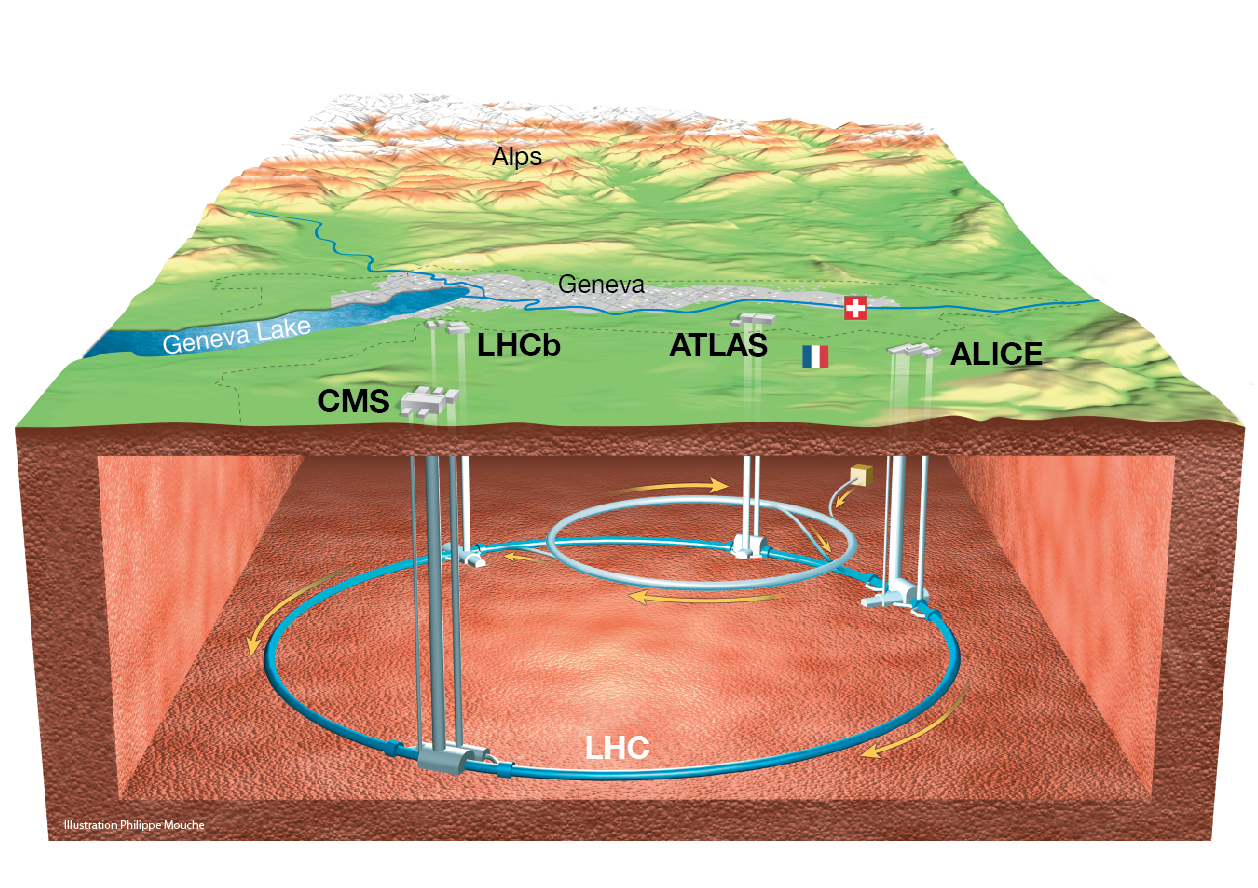
\includegraphics[width=4in]{images/LHC-illustration}
    \caption[Overall View of the LHC]{An overall view of the LHC showing the underground tunnel and its experiments in relation to its geography.\cite{LHCoverallview}}
    \label{fig:LHCoverallview}
\end{figure}

Because the LHC reuses the tunnels of the Large Electron-Positron (LEP) Collider, additional excavation was avoided and it was integrated as the final stage of CERN's accelerator complex, shown in Figure \ref{fig:CERNcomplex}. The source of protons is a canister of hydrogen gas to which a strong electric field is applied to strip the electrons from the hydrogen nuclei. The protons then pass through the linear accelerator LINAC2 and are accelerated to an energy of 50 \MeV. They are then injected into successive circular accelerators: the Proton Synchrotron Booster which accelerates the beams to 1.4 \GeV, the Proton Synchrotron (PS) which accelerates the beams to 25 GeV, the Super Proton Synchrotron (SPS) which further accelerates the beams to 450 \GeV, and finally the LHC itself. The oscillating radio frequency (RF) fields used to accelerate the protons results in beams composed of proton \textit{bunches} as opposed to a continuous stream. The LHC currently circulates up to 2556 bunches per beam, which is not far from its design value of 2808 bunches per beam.

\begin{figure}[htbp]
  \centering
    \includegraphics[width=6.5in]{images/CERNcomplex}
    \caption[CERN Accelerator Complex]{A complete schematic of the CERN accerlator complex and experiments.\cite{CERNcomplex}}
    \label{fig:CERNcomplex}
\end{figure}

The circular orbit of the proton beams are maintained by the 1,232 bending magnets lining the LHC. The bending magnets are superconducting dipole magnets which generate 8.3 T magnetic fields powerful enough to bend the high energy beams. In order to minimize the oscillation of the bunches around their trajectories and achieve high luminosity, 392 focusing magnets are also placed along the LHC ring. The focusing magnets are superconducting quadrupole magnets with a magnetic field gradient of 223 T/m. They are placed in alternating pairs to account for their nature of focusing along one direction while defocusing the orthogonal direction. Schematics for these two main types of magnets are shown in Figure \ref{fig:lhcmagnets}. In order to maintain the superconductivity of these magnets, the cryogenic systems cool them down to a temperature of 1.9 K.

\begin{figure}[htbp]
  \centering
  \mbox{
    \subfigure [] {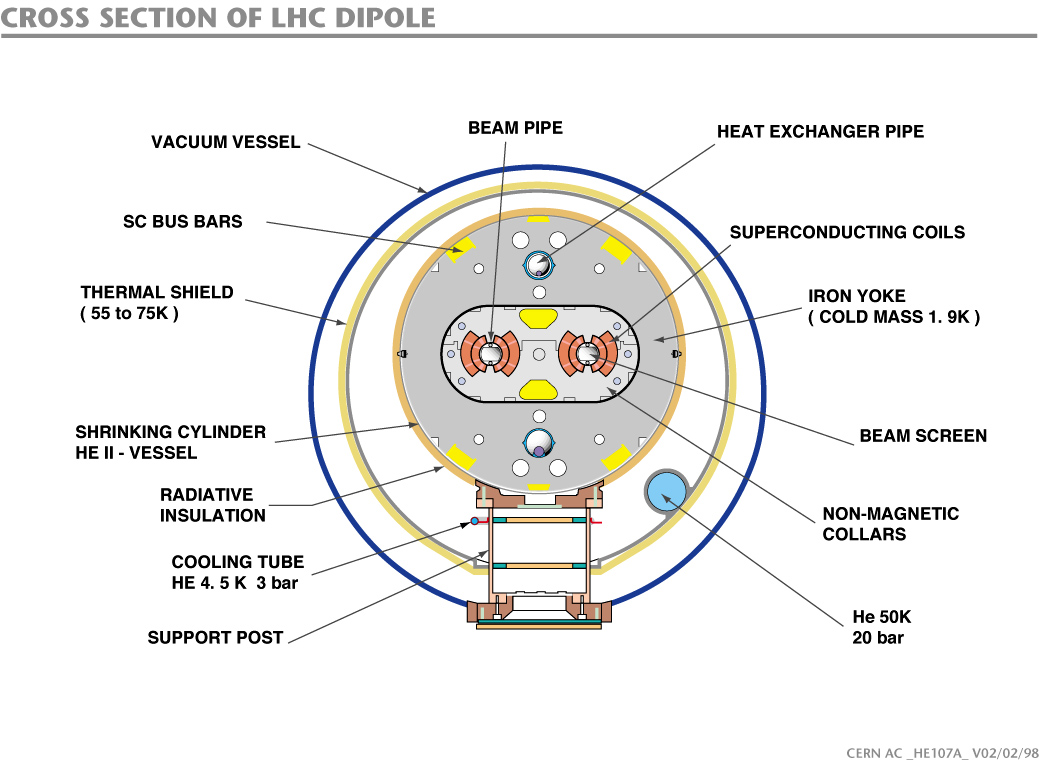
\includegraphics[scale=0.27]{images/lhc-pho-1998-341}} \qquad
    \subfigure [] {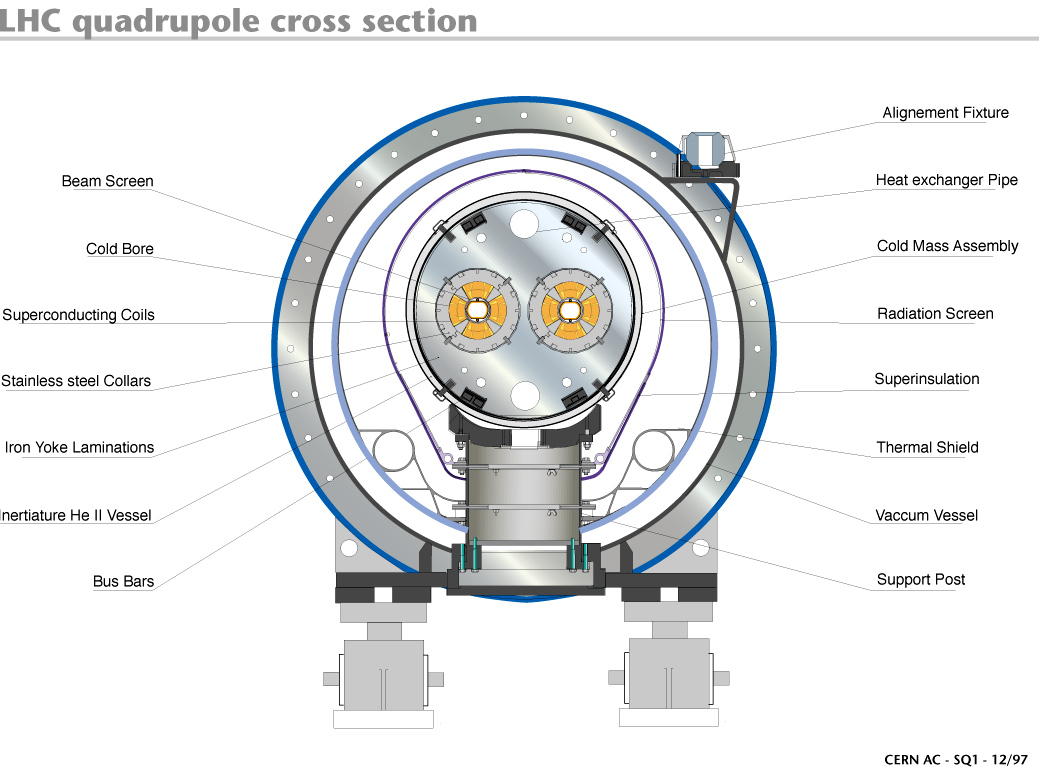
\includegraphics[scale=0.27]{images/lhc-pho-1998-312}} \qquad
  }
  \caption[LHC Dipole and Quadrupole Magnets]{The cross sectional views for the main types of LHC magnets: A) dipole magnet used for bending the beams; B) quadrupole magnet used for focusing the beams.\cite{dipole,quadrupole}}
  \label{fig:lhcmagnets}
\end{figure}

The beams are directed to cross through each other at four sites around the LHC known as interactions points. At these points, fine control of the beam is crucial because it has direct ramifications on the number of possible interactions. The interaction rate of any given process is proportional to its cross section $\sigma$ and the luminosity $\mathcal{L}$ of the collider
\begin{equation}
  \frac{dN}{dt} = \sigma\mathcal{L},
\end{equation}
where $N$ refers to the number of interactions. The cross section, or interaction probability, is fixed by physics while the luminosity is determined by the collider's design, and therefore the highest possible luminosity is desired in order to observe rare interactions such as those that produce Higgs bosons. For equal, bunched beams with a rounded profile, the luminosity can be expressed as
\begin{equation}
  \mathcal{L} = \frac{ N^{2} k_{b} f \gamma }{ 4 \pi \epsilon_{n} \beta^{\ast} } F,
\end{equation}
where the various parameters are determined by the design of the collider: $N$ is the number of protons per bunch, $k_{b}$ is the number of bunches, $f$ is the revolution frequency, $\gamma$ is the typical Lorentz factor, $\epsilon_{n}$ is the normalized emittance, $\beta^{\ast}$ is the value of the betatron function at the interaction point, and $F$ is the geometrical reduction factor due to the crossing angle.\cite{CMSTDR1}

The LHC has a 25 ns bunch spacing, or time between bunch crossings at the interaction point, which places a constraint on how large $k_{b}$ and $f$ can be. The spacing cannot be lowered due to operational safety concerns, such as providing kicker magnets enough time to ramp up and divert the bunches toward a beam dump for absorption. The normalized emittance $\epsilon_{n}$ is a measure of the kinematic phase space occupied by the particles in the bunch and can be improved by reducing the size of the bunch and the spread in momentum of its particles. The beta function is a measure of the beam's transverse size and so its value at the interaction point $\beta^{\ast}$ is determined by how well the magnets can focus the beam at the interaction point. The geometrical factor $F$ corrects the amount by which the colliding bunches overlap as they are made to cross at a shallow angle. While a head-on collision would result in the greatest overlap, it also increases the chances of long range electromagnetic interactions between bunches, so there is some interplay in determining the crossing angle.

Although the design luminosity of the LHC is $10^{34}\ \mathrm{cm}^{-2} \mathrm{s}^{-1}$, it has exceeded expectations by achieving a luminosity of twice the designed value. As a measure of particle flux, the luminosity that has been discussed so far is a dynamic quantity and is better called \textit{instantaneous luminosity}. The expected number of interactions $N$ for a specific process is thus given by
\begin{equation}
  N = \sigma \int \mathcal{L}dt = \sigma \mathcal{L}_{int},
\end{equation}
where $\mathcal{L}_{int}$ is the \textit{integrated luminosity}, and so the total integrated luminosity is quoted in reference to the size of particle physics datasets.

Surrounding each of the interaction points of the LHC are its four main experiments: A Large Ion Collider Experiment (ALICE), A Toroidal LHC ApparatuS (ATLAS), the Compact Muon Solenoid (CMS), and the Large Hadron Collider beauty (LHCb). Both ATLAS and CMS are general-purpose detectors designed to search for the Higgs boson and perform precise measurements of its properties, while also exploring the new energy frontier in search of physics beyond the Standard Model. The LHC can also accelerate lead ions, which is used by ALICE to study heavy-ion collisions and the dynamics of quark-gluon plasma. As general-purpose detectors, ATLAS and CMS also study heavy-ion collisions. The LHCb experiment specializes in studying the electroweak and QCD physics of heavy flavor quarks and measuring the properties of B mesons.

\section{The Compact Muon Solenoid}

The Compact Muon Solenoid (CMS), illustrated in Figure \ref{fig:CMScutaway}, is a general-purpose particle detector and one of the two main experiments at the LHC. Its cylindrical design is impressively compact for its purpose, with a diameter of 15 m and a length of 28.7 m. Although heavy, weighing in at 14,000 tonnes, the bulk of this weight comes from its steel return yoke and structural supports which together weigh 12,500 tonnes. The return yoke guides and contains the 3.8 T magnetic field generated by the detector's namesake superconducting solenoid, which is cooled by its cryostat to a temperature of 4.5 K during operation.

\begin{figure}[htbp]
  \centering
    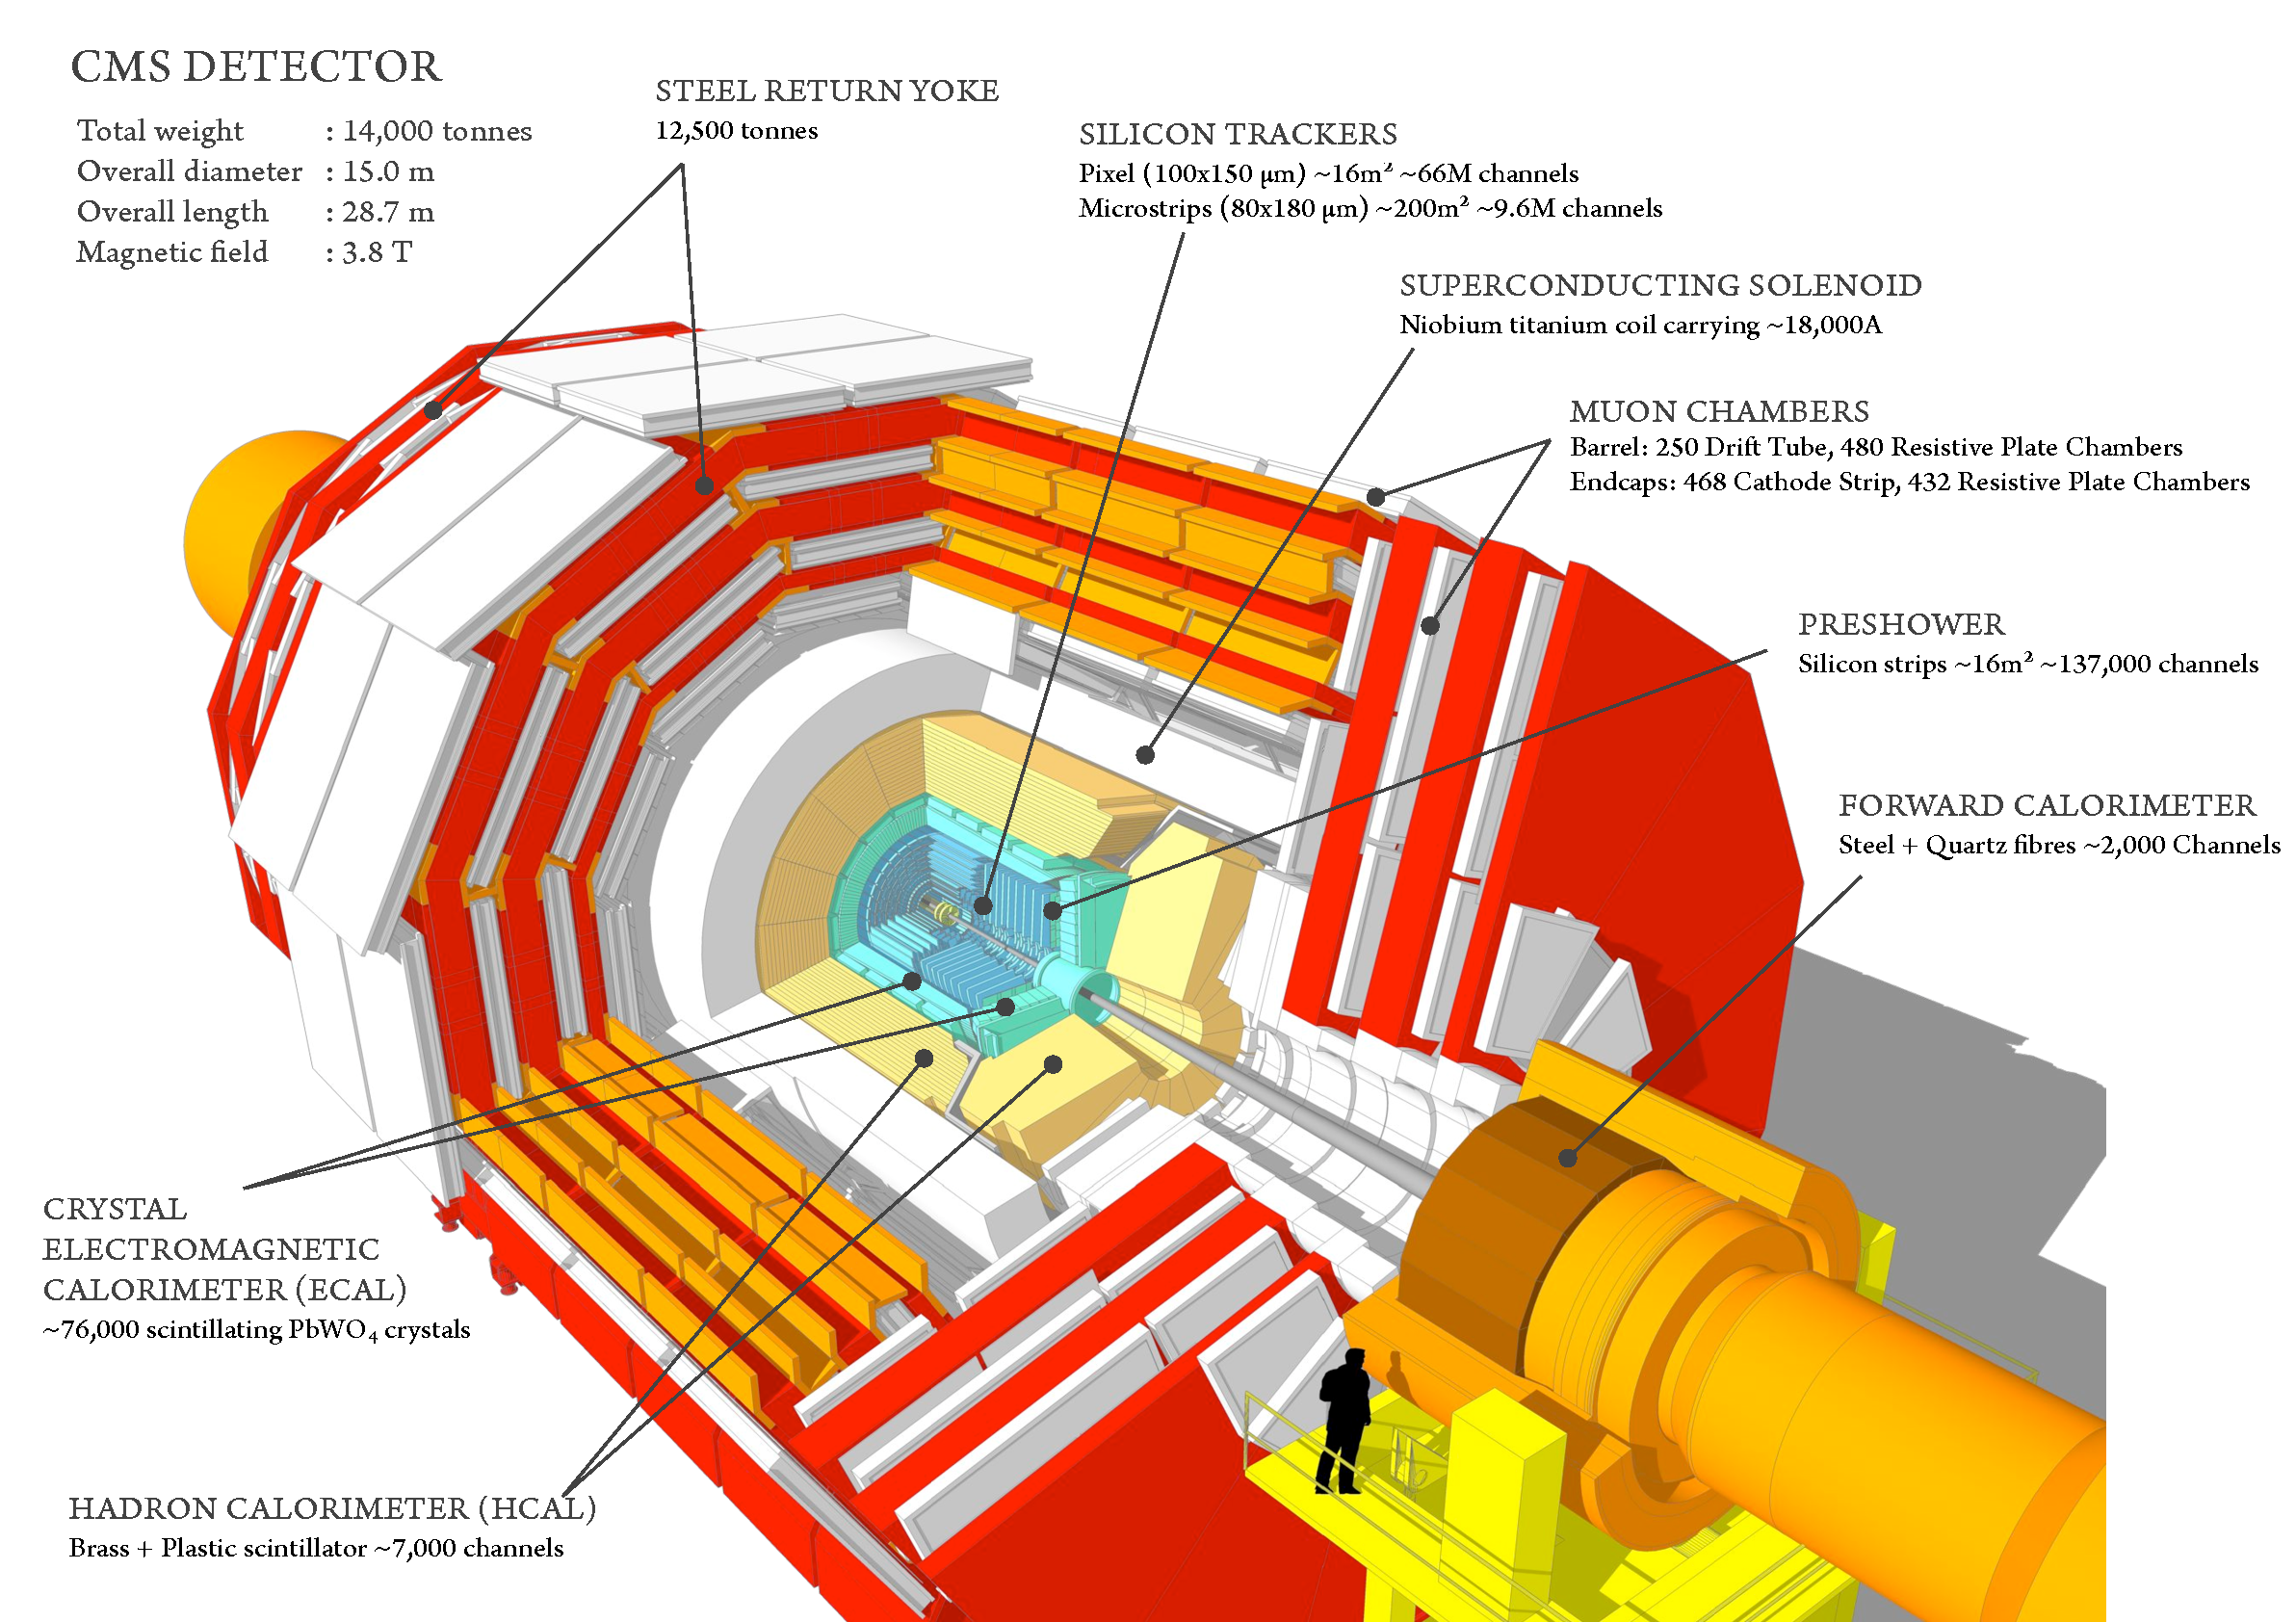
\includegraphics[width=5.5in]{images/cms_120918_03}
    \caption[Cutaway View of the CMS Detector]{A cutaway view of the CMS detector with its main subsystems and components labeled.\cite{CMScutaway}}
    \label{fig:CMScutaway}
\end{figure}

The solenoid is central to the design of the CMS detector because it provides a uniform magnetic field capable of bending the trajectories of charged particles as they travel through the detector, thereby enabling the measurement of their electric charge and transverse momentum \pT. This follows because a particle with electric charge $q$ and velocity $\mathbf{v}$ moving through a uniform magnetic field $\mathbf{B}$ experiences a Lorentz force given by
\begin{equation}
  \mathbf{F} = q\mathbf{v} \times \mathbf{B}.
\end{equation}
Since the force is transverse to the direction of motion, the particle travels along a helical path of radius $R$ with a handedness determined by its electric charge. An application of Newton's 2\textsuperscript{nd} Law upon the circular motion of such a particle with mass $m$ and velocity transverse to the direction of motion $v$ further shows that its transverse momentum is determined by the radius of curvature of its path
\begin{equation}
  \frac{mv^{2}}{R} = qvB \implies \pT = qRB,
\end{equation}
where $\pT = mv$ is the transverse momentum of the particle.

While the helical paths of charged particles travelling with low momentum are fully contained within the detector, the trajectories of charged particles with high momentum are recorded as incomplete arcs, either because they decay mid-flight or, in the case of muons, travel out of the detector. While the radius of curvature of such highly energetic particles cannot be directly measured, it can be obtained by measuring the sagitta of their \textit{track}, the arc they trace through the detector.

\begin{figure}[htbp]
  \centering
    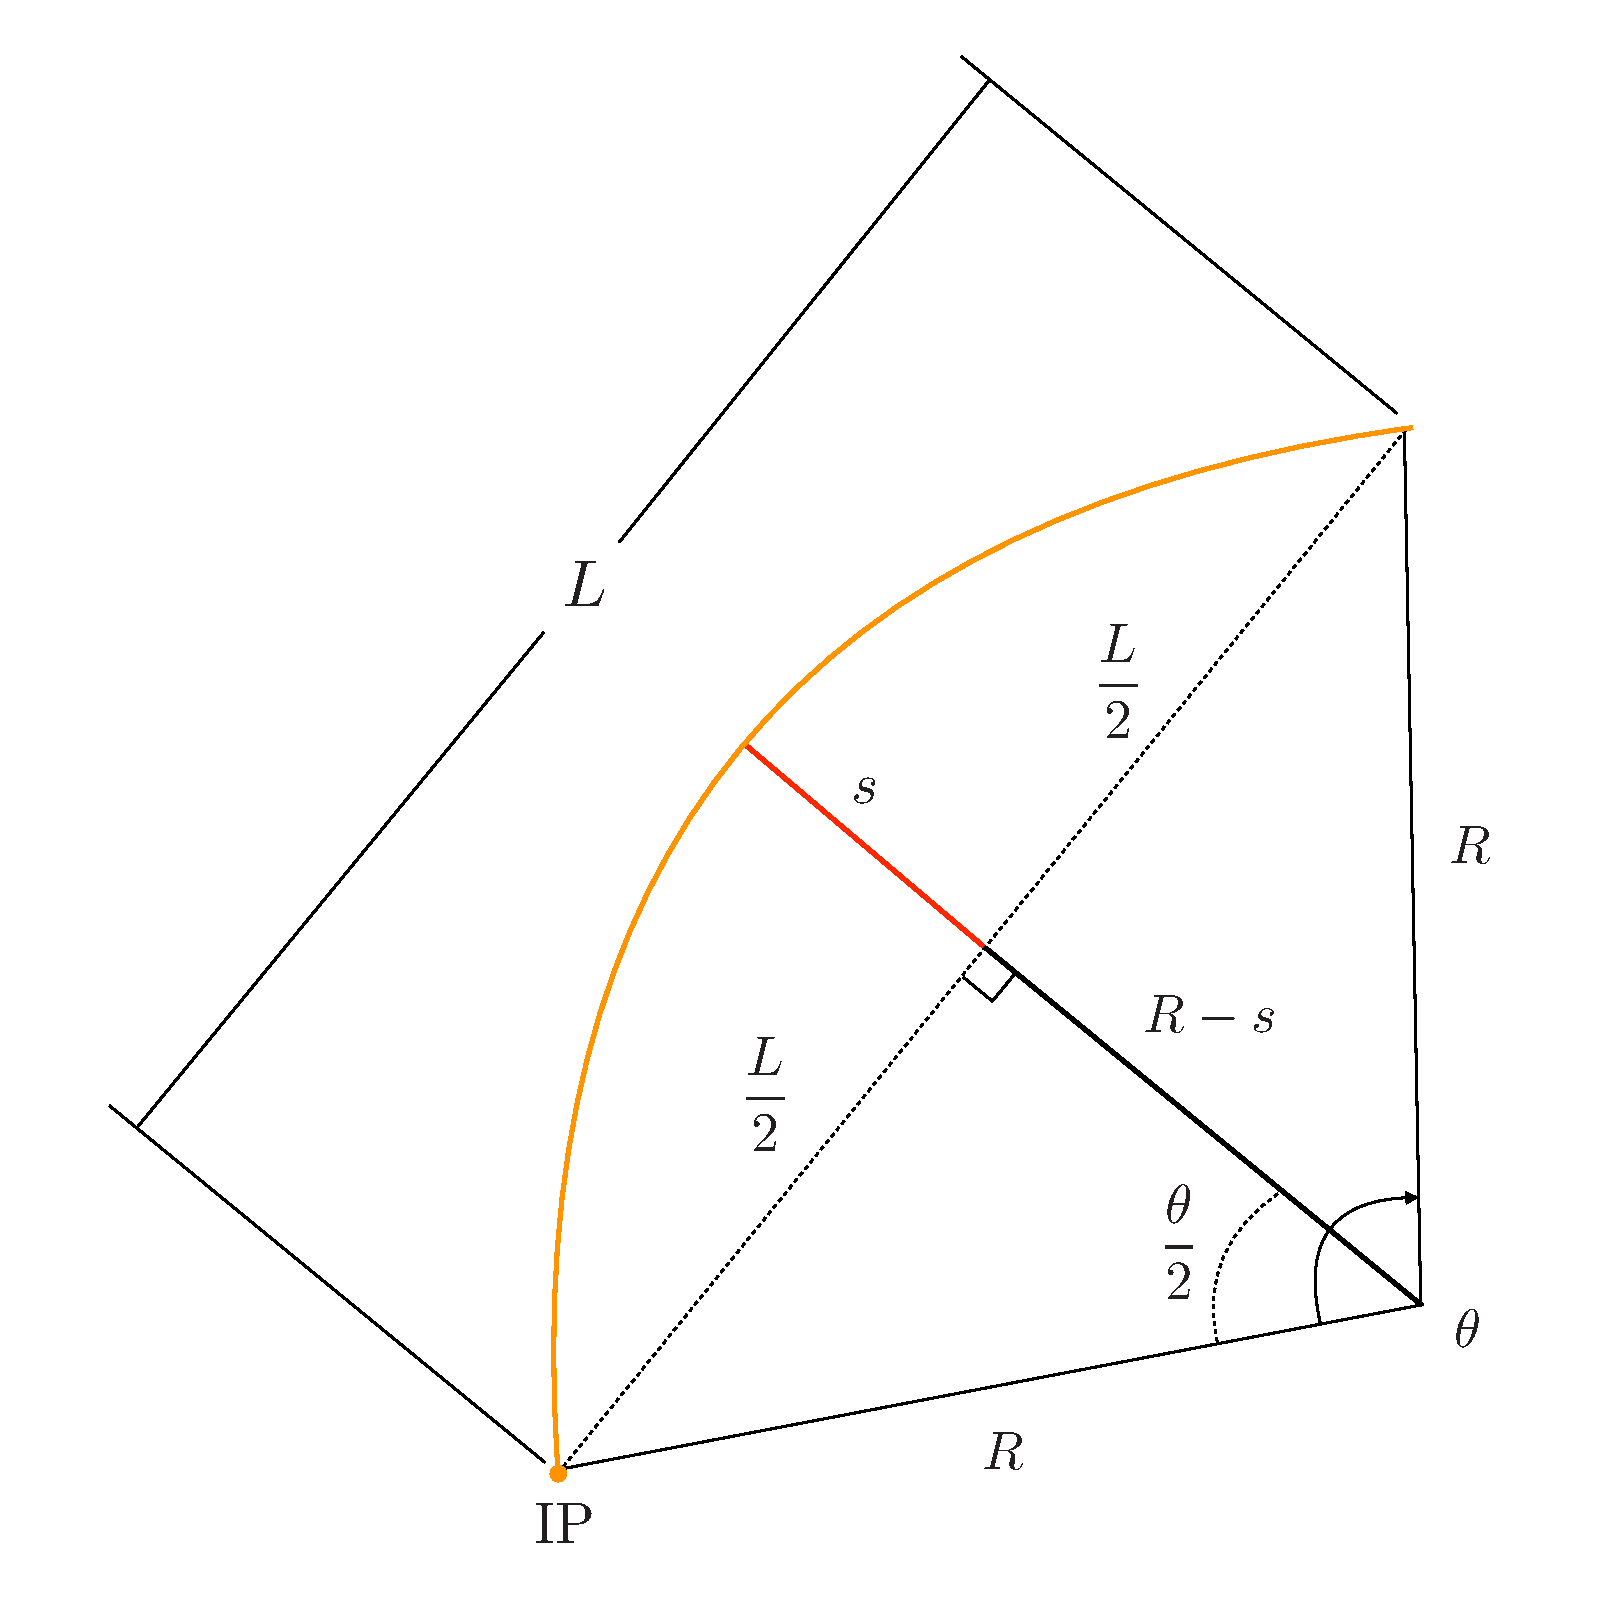
\includegraphics[width=4in]{images/sagitta}
    \caption[Sagitta of a Charged Particle Track]{A diagram defining the sagitta of an arc representing a charged particle track (orange) travelling away from the interaction point (IP). The track has a chord of length $L$, an opening angle of $\theta$, a radius of curvature $R$, and a sagitta (red) of length $s$.}
    \label{fig:sagitta}
\end{figure}

From Figure \ref{fig:sagitta}, a relationship between the chord length $L$, radius of curvature $R$, and sagitta $s$ of the track can be constructed using the Pythagorean Theorem such that
\begin{equation}
  R^{2} = \left( R - s \right)^{2} + \left( \frac{L}{2} \right)^{2}.
\end{equation}
Solving for $R$ with the reasonable assumption that $s \ll L$ yields
\begin{equation}
  R = \frac{L^{2}}{8s} + \frac{s}{2} \approx \frac{L^{2}}{8s},
\end{equation}
and therefore the \pT\ of a charged particle can be determined from the chord length and sagitta of its track
\begin{equation}
  \pT = \frac{qBL^{2}}{8s}.
\end{equation}
The magnetic field strength $B$ and, in part, the chord length $L$ are dictated by the design of the detector, and so the \pT\ resolution is limited by the resolution of the sagitta. As their momentum increases, charged particles leave straighter tracks which make it difficult to accurately measure the sagitta, thereby degrading the resolution at high momentum.

Because the magnetic field within the solenoid is oriented along the direction of the beam, it motivates the coordinate system adopted for the CMS detector that is shown in Figure \ref{fig:CMS_coord_sys}. The geometrical center of the detector defines the origin of the right-handed Cartesian coordinate system with the \textit{z}-axis oriented along the direction of the anticlockwise proton beam from the LHC, the \textit{x}-axis pointing horizontally towards the center of the LHC ring, and the \textit{y}-axis pointing vertically upwards out of the plane of the LHC ring. The shape of the detector also permits a cylindrical description about the same origin. With the \textit{x}-axis and \textit{z}-axis taken to be the polar and longitudinal axes, respectively, a cylindrical coordinate system can be defined with the azimuthal angle $\phi$ taken with respect to the positive \textit{x}-axis ($\phi = 0$) and the polar angle $\theta$ taken with respect to the positive \textit{z}-axis ($\theta = 0$). Because the polar angle $\theta$ is not Lorentz invariant under boosts along the direction of the beam, it is typically transformed into the \textit{pseudorapidity}
\begin{equation}
  \eta = -\ln\left[\tan\left(\frac{\theta}{2}\right)\right]
\end{equation}
such that the positive \textit{z}-axis has $\eta = + \infty$ and the positive \textit{y}-axis has $\eta = 0$.

\begin{figure}[htbp]
  \centering
    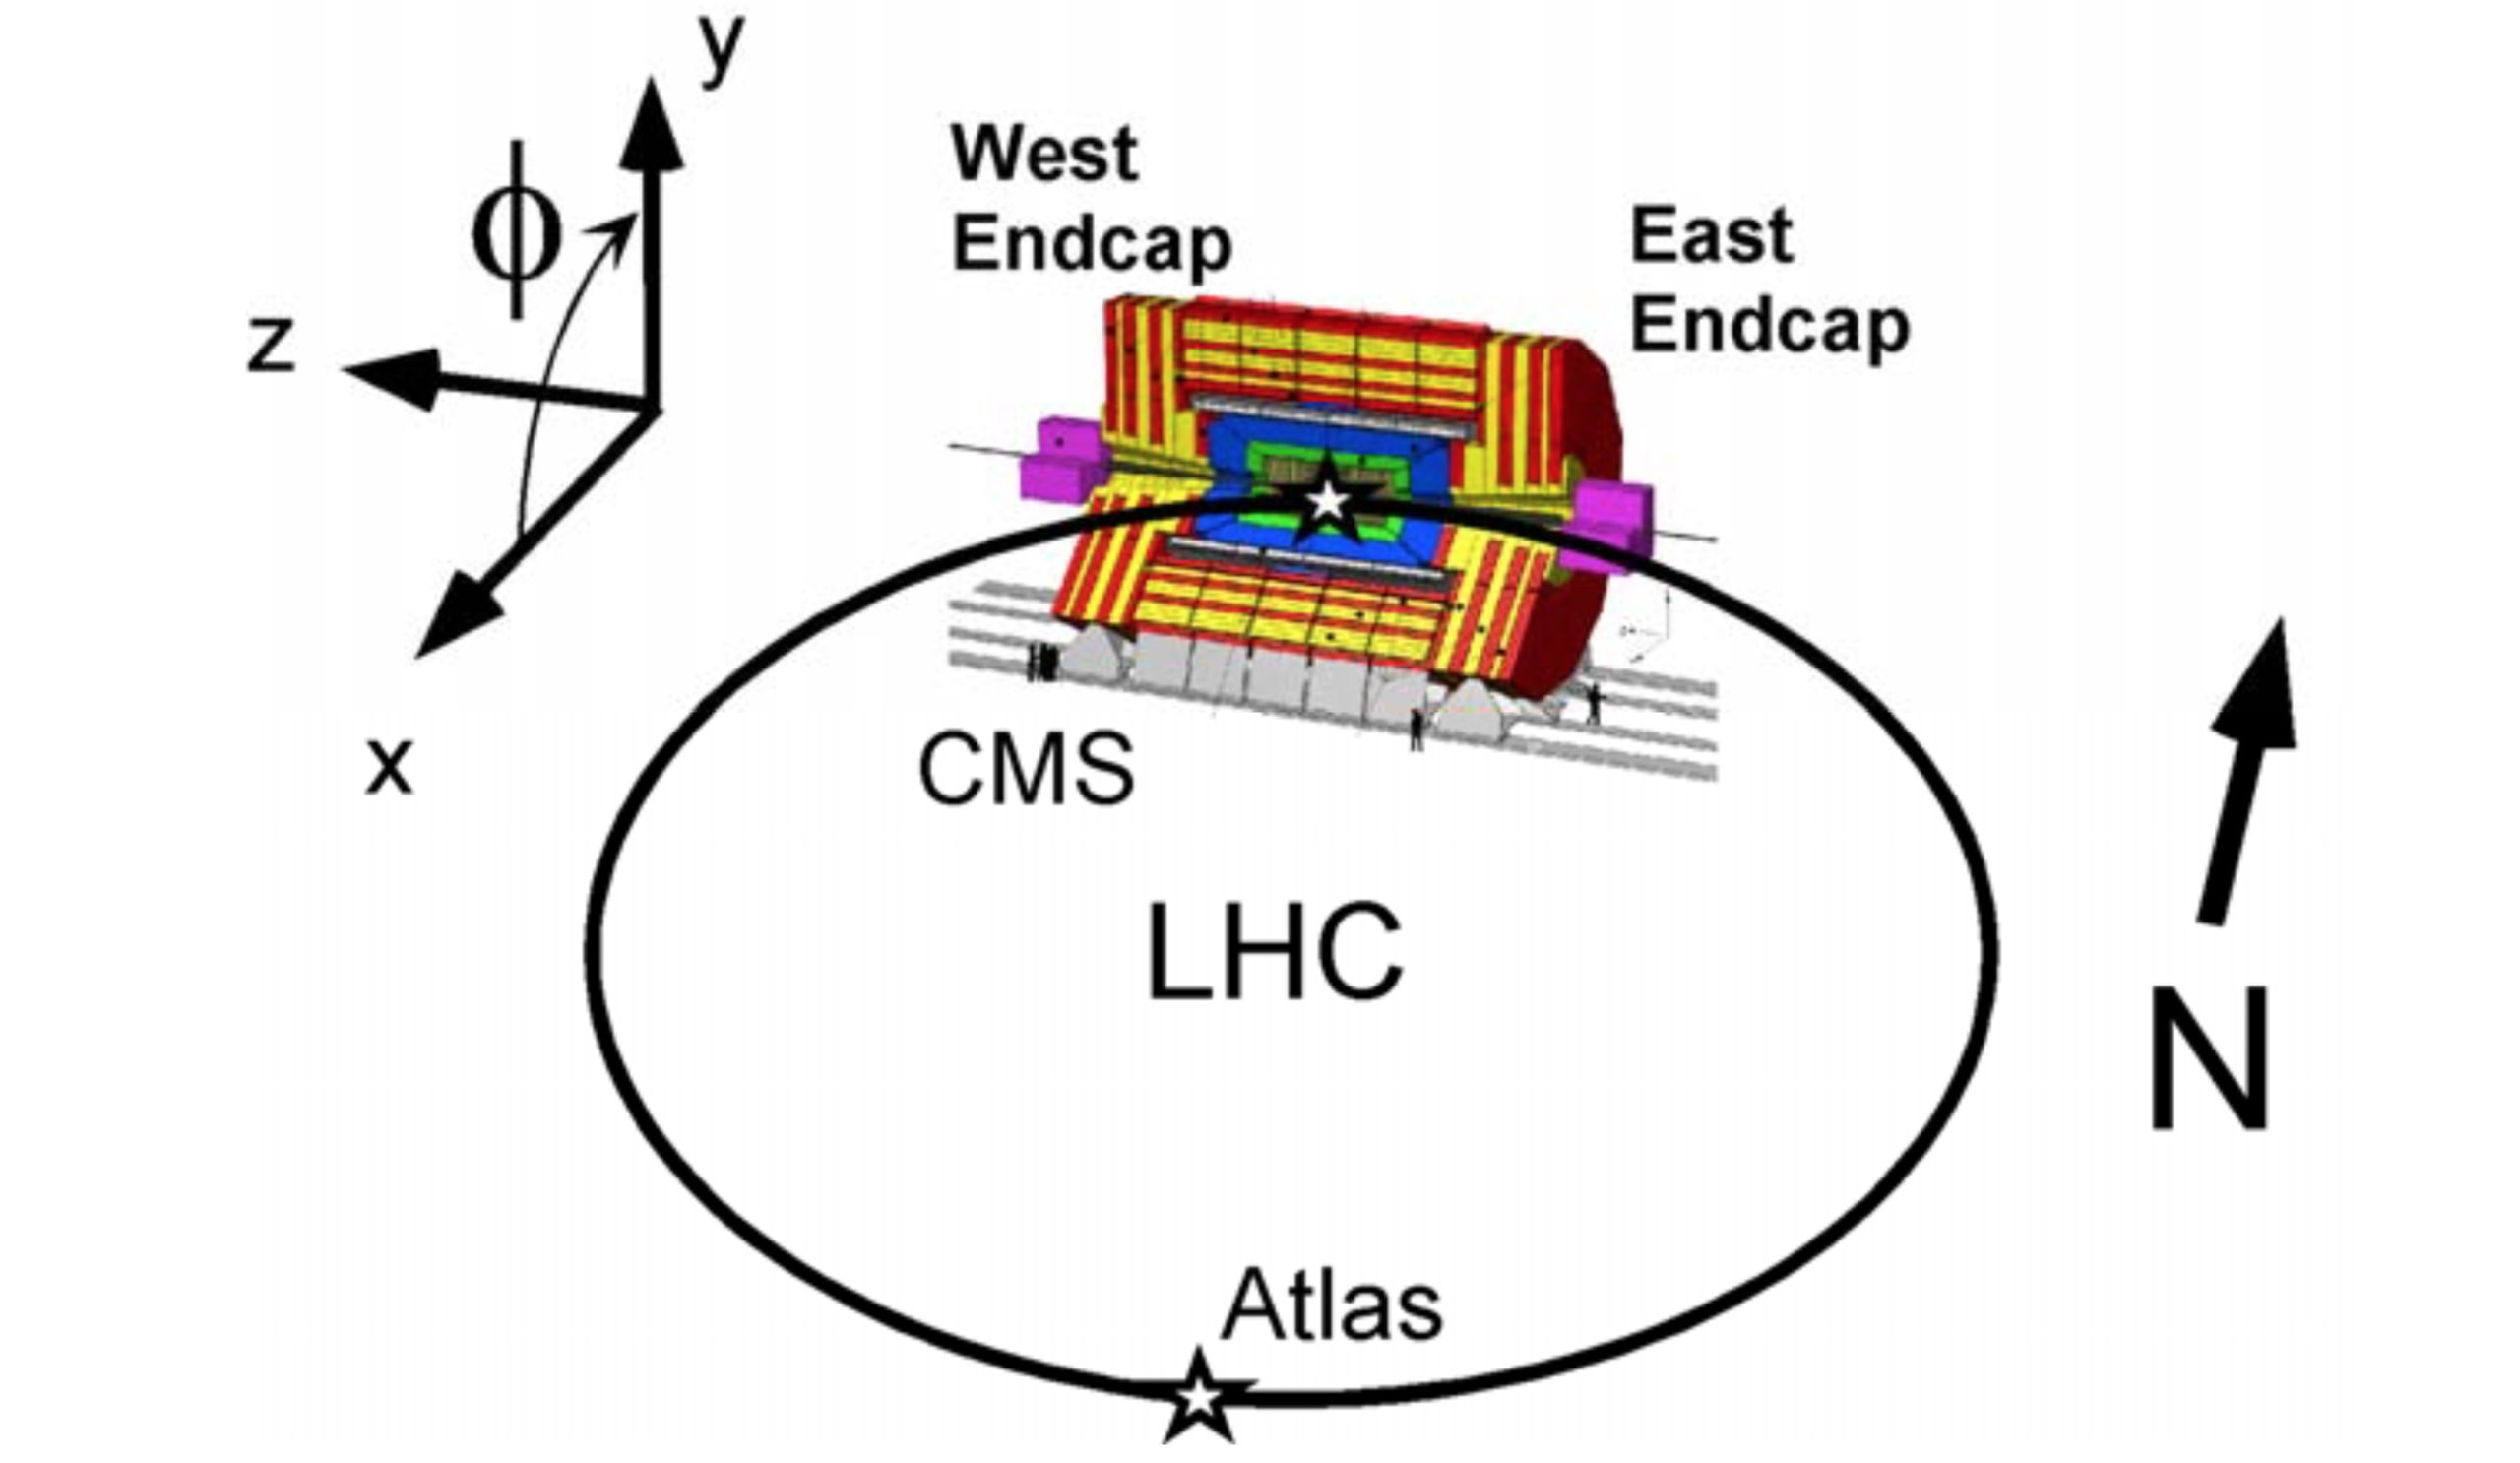
\includegraphics[width=4in]{images/CMS_coord_sys}
    \caption[Coordinate System of the CMS Detector]{The coordinate system convention used for the CMS detector.\cite{CMSCoordSys}}
    \label{fig:CMS_coord_sys}
\end{figure}

\subsection{Detector Subsystems}

As with all modern general-purpose detectors, the guiding principle in the design of the CMS detector is hermeticity. By maximizing the angular coverage of the space surrounding the interaction point, the final state particles produced by proton-proton collisions are more likely to be recorded by the detector's subsystems. The CMS detector is composed of layered subsystems as illustrated in Figure \ref{fig:CMSslice}, each designed to detect and measure the properties of different types of particles. Each of the detector subsystems are described in the following sections, starting from those closest to the interaction point. A thorough discussion of the detector's design is available in Ref. \cite{CMSTDR1}, the first volume of the official CMS Technical Design Report (TDR).

\begin{figure}[htbp]
  \centering
    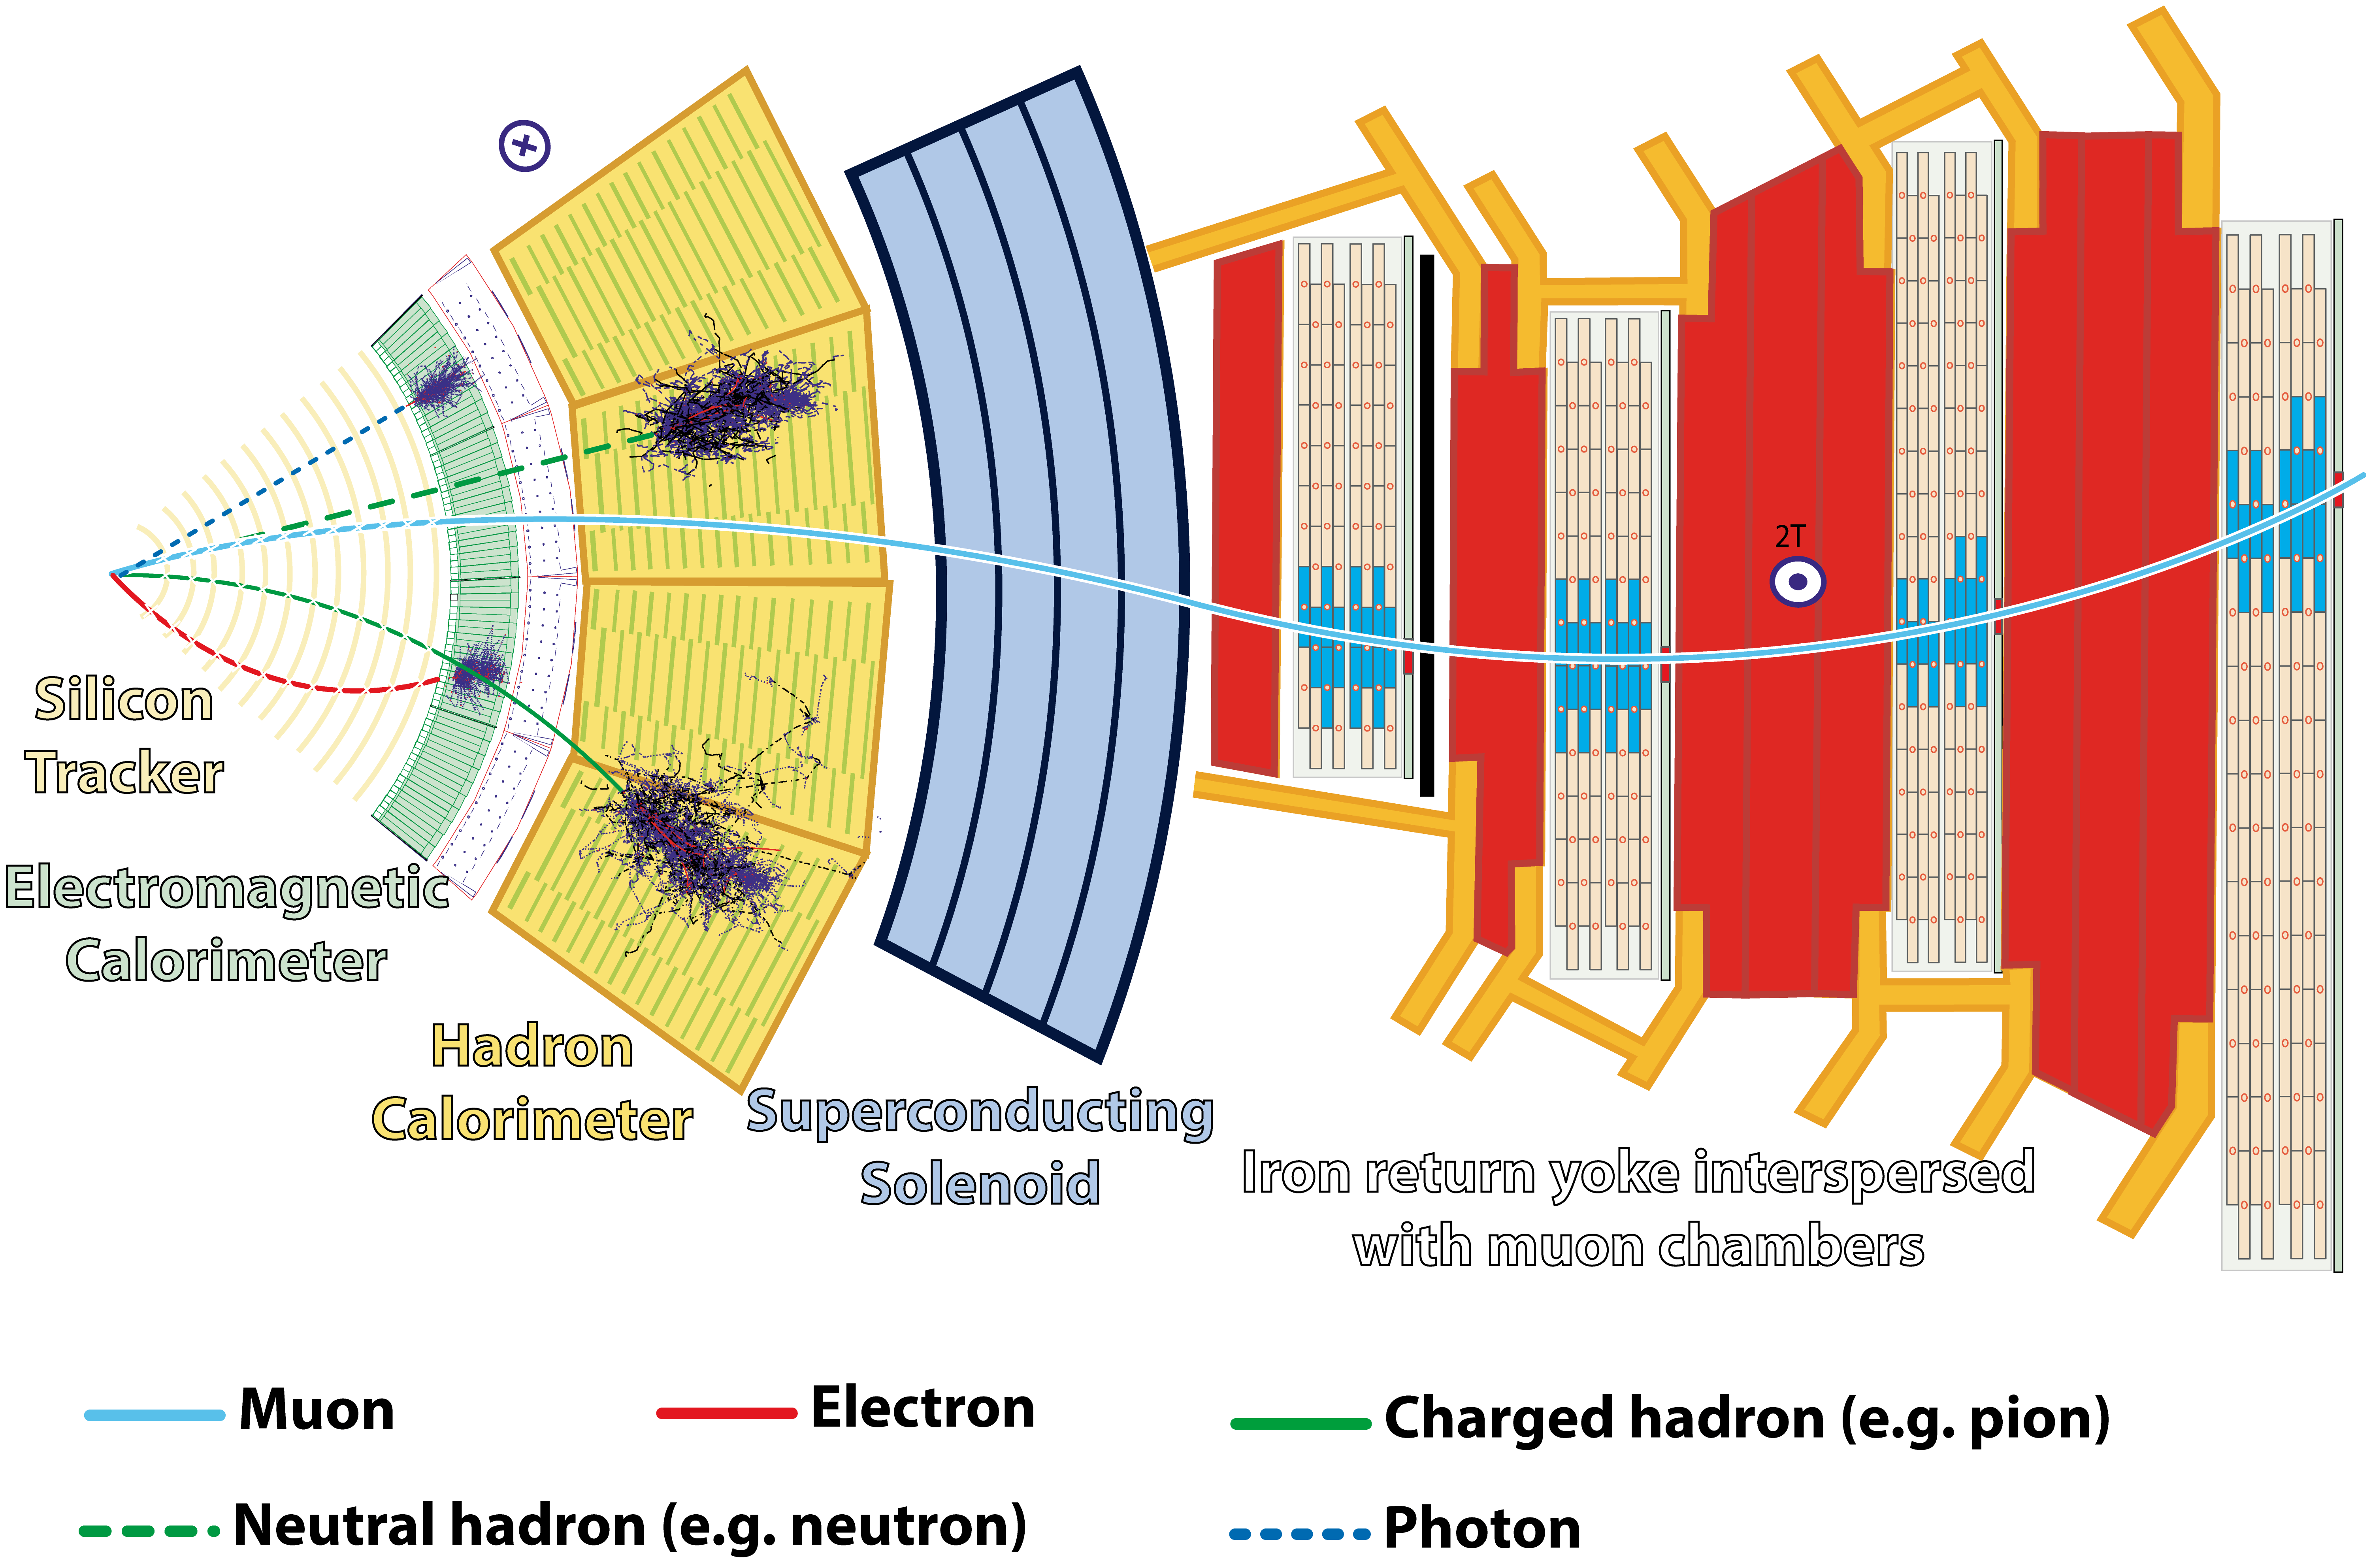
\includegraphics[width=5.5in]{images/CMSslice_whiteBackground}
    \caption[Cross Sectional View of the CMS Detector]{A cross sectional view of the CMS detector in the $r\phi$-plane revealing the different subsystems and the particles they are used to detect.\cite{CMSslice}}
    \label{fig:CMSslice}
\end{figure}

\subsubsection{Silicon tracker}

\begin{figure}[htbp]
  \centering
    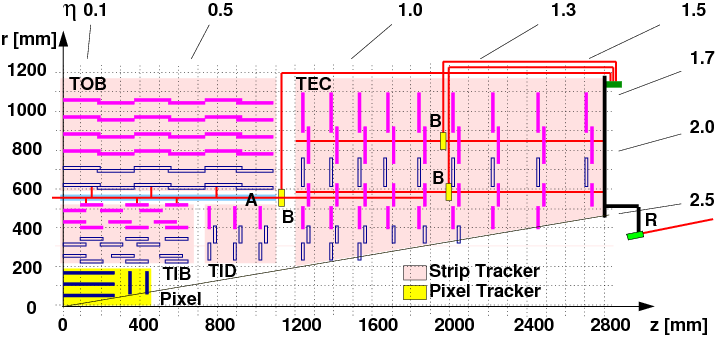
\includegraphics[width=5.5in]{images/tracker_diagram}
    \caption[Schematic for the CMS Silicon Tracker]{A schematic diagram showing a cross sectional view of the CMS detector's silicon tracker in the positive $yz$-plane.\cite{TRACKERDIAGRAM}}
    \label{fig:CMStrackerdiag}
\end{figure}

The tracker is designed to detect charged particles and measure their trajectories or ``tracks''. As the innermost layer surrounding the interaction point, its components must have a fast response time to record the tracks of short-lived particles, good spatial resolution to distinguish between tracks of different particles, and excellent radiation tolerance to withstand the high intensity of the proton beams. These concerns motivated the choice of semiconductor detectors made from silicon, which offer fast response times and excellent energy resolution and acceptable radiation hardness, although degradation is expected over time. When a charged particle passes through a semiconductor module, valence band electrons are promoted to the conduction band and leave behind ``holes''. By applying an electric field, the electrons and holes are collected by electrodes to generate a signal indicating the passage of a charged particle. 

The tracker is composed of 16,588 silicon modules distributed between the pixel tracker, which segments its sensors into 66 million pixels of size $100 \times 150 \mu\mathrm{m}^{2}$\footnote{For reference, the average width of a human hair is around 100 $\mu\mathrm{m}$.}, and strip tracker, which segments its sensors into 9.6 million strips that are 80 to 180 $\mu\mathrm{m}$ wide. The tracker is divided into four regions as shown in Figure \ref{fig:CMStrackerdiag}, with the inner barrel (TIB) and outer barrel (TOB) arranged in cylindrical layers and the inner disks (TID) and endcaps (TEC) arranged in layered disks. This offers full angular coverage in $\phi$ and $\left| \eta \right| < 2.5$, and the granularity of the pixels and strips achieves a \pT\ resolution of approximately 1.5\% for charged particles with $1\ \GeV < \pT < 10\ \GeV$ in the central region of the tracker.\cite{CMSTRACKERPERF}

\subsubsection{Electromagnetic calorimeter}

\begin{figure}[htbp]
  \centering
    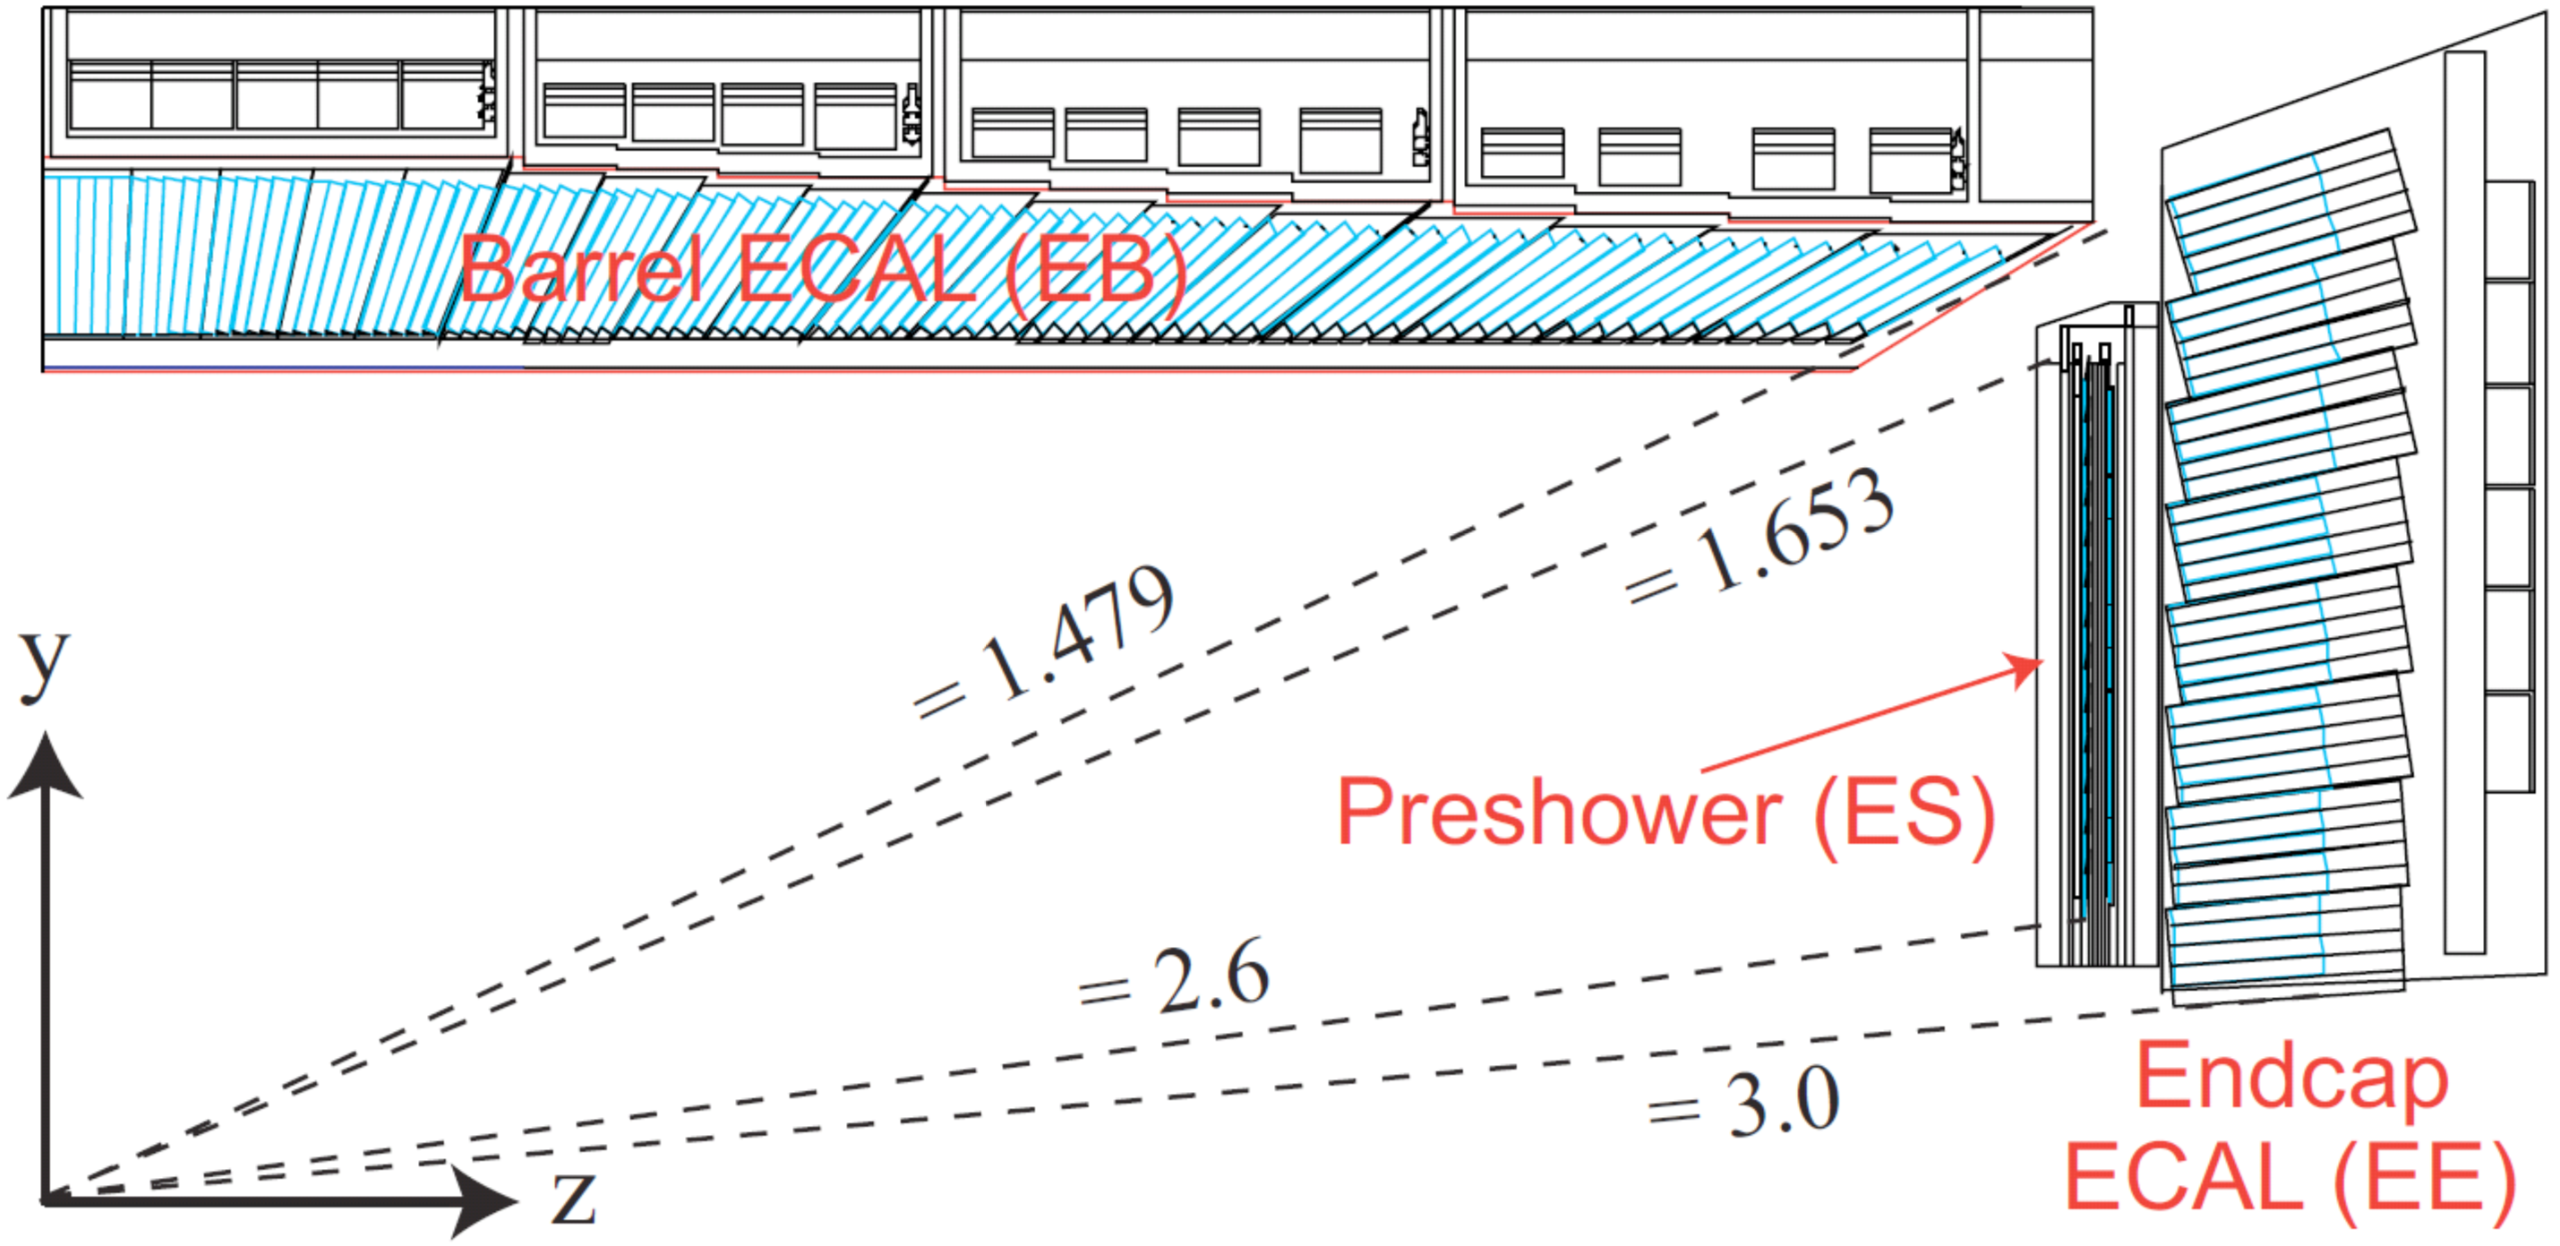
\includegraphics[width=5.5in]{images/ecal_diagram}
    \caption[Schematic for the CMS ECAL]{A schematic diagram showing a cross sectional view of the CMS detector's electromagnetic calorimeter in the positive $yz$-plane.\cite{ECALDIAGRAM}}
    \label{fig:CMSecaldiag}
\end{figure}

The electromagnetic calorimeter (ECAL) is designed to detect electrons and photons based on their energy deposition. When highly energetic electrons or photons interact with matter, they initiate an electromagnetic shower via bremsstrahlung or electron-positron pair production, respectively. Because these secondary particles may interact further with the material, the electromagnetic shower proceeds until the energies of the produced particles fall below a critical energy and energy losses proceed through ionization. If the material is a scintillator, it can absorb the low energy particles produced by the shower and produce an amount of light proportional to their energies that can be measured by photodetectors.

To ensure that the energies of incident electrons and photons are collected by the ECAL, lead tungstate ($\mathrm{PbWO}_{4}$) crystals were chosen for their low radiation length and Moli{\`e}re radius, fast response, and radiation hardness. The radiation length is the mean distance over which a particle radiates approximately 63\% of their energy, while the Moli{\`e}re radius specifies the radius of the cylindrical volume that contains approximately 90\% of the energy of the incident electron or photon. By selecting a material that minimizes both of these properties, the full absoprtion of electrons and photons can be achieved within a limited material budget.

The ECAL is composed of 75,848 lead tungstate crystals distributed between the ECAL barrel (EB) which uses 61,200 crytals and the ECAL endcap (EE) which uses 14,648 crystals, as shown in Figure \ref{fig:CMSecaldiag}. The additional ECAL preshower (EC) layer is placed before the EE and consists of alternating lead and silicon modules instead of lead tungstate crystals. The finer granularity of the EC is used to reject closely-spaced photon pairs produced by the decay of neutral pions based on their energy deposits, which could otherwise be identified as a high energy photon by the ECAL. On the whole, the ECAL offers full angular coverage in $\phi$ and $\left| \eta \right| < 3.0$ and achieves an energy resolution between 2-5\% for electrons and 1.1-5\% for photons.\cite{CMSECALPERF}

\subsubsection{Hadronic calorimeter}

\begin{figure}[htbp]
  \centering
    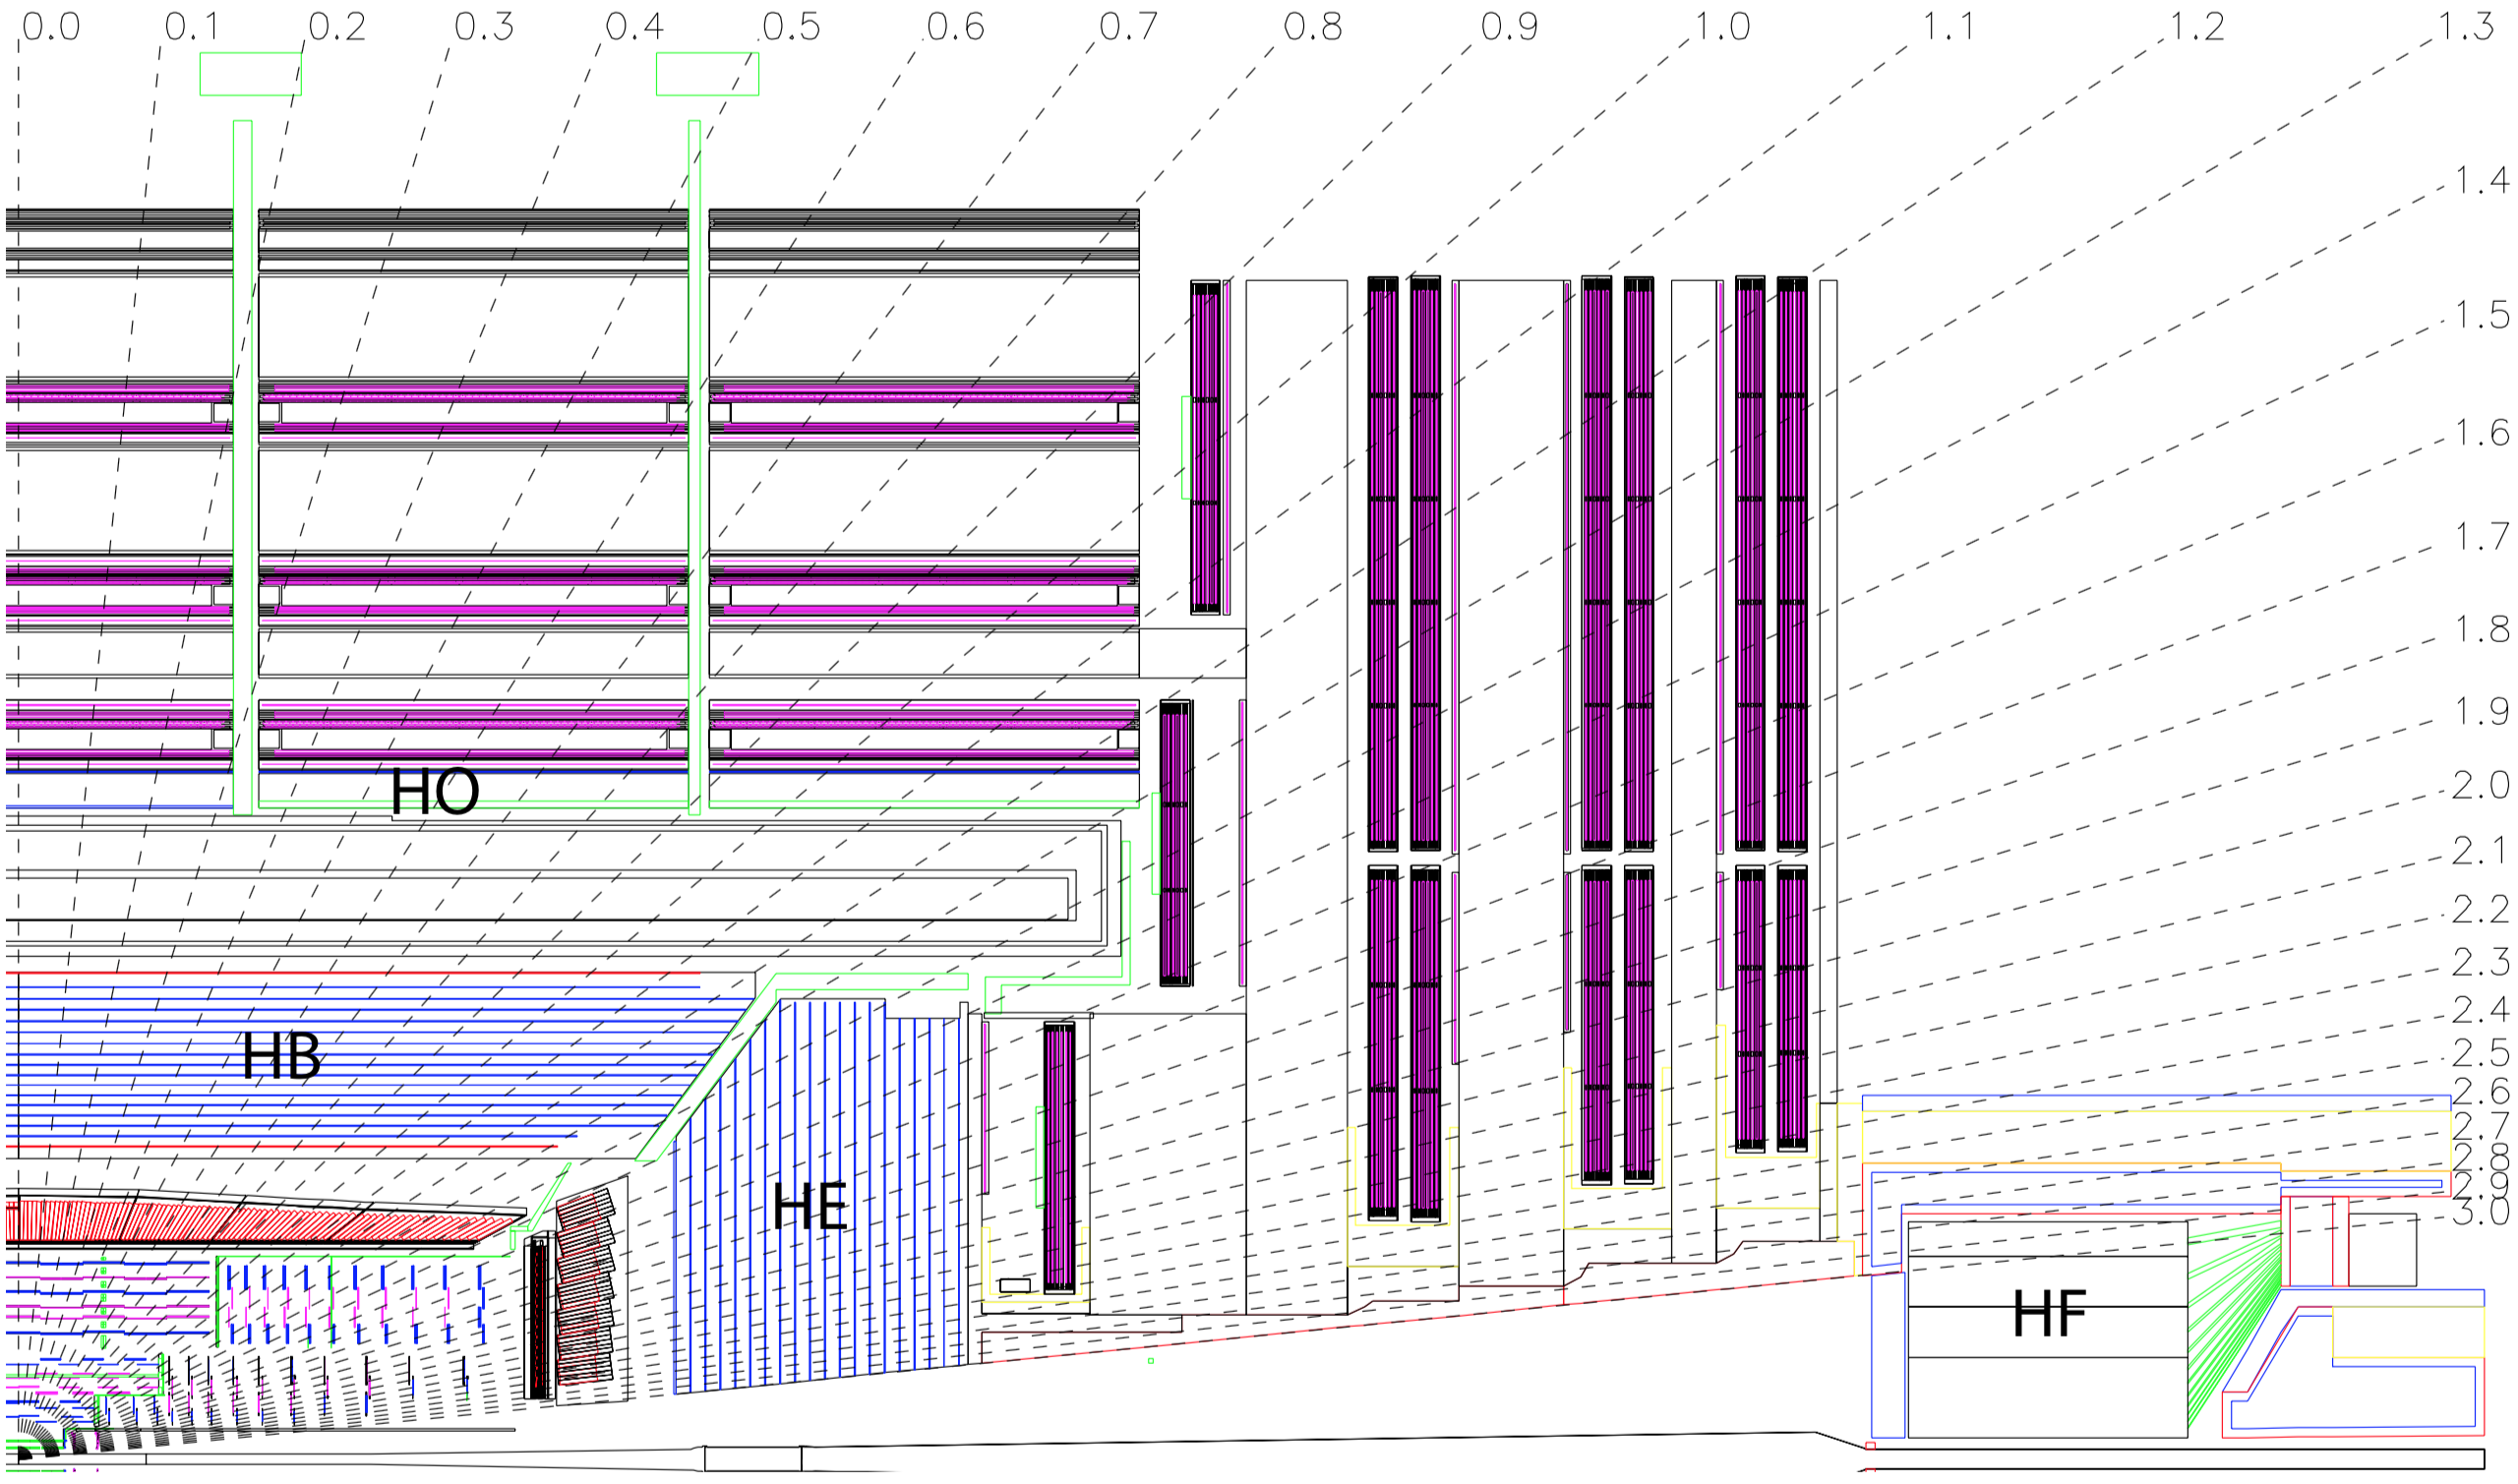
\includegraphics[width=5.5in]{images/hcal_diagram}
    \caption[Schematic for the CMS HCAL]{A schematic diagram showing a cross sectional view of the CMS detector's hadronic calorimeter in the positive $yz$-plane.\cite{HCALDIAGRAM}}
    \label{fig:CMShcaldiag}
\end{figure}

The hadronic calorimeter (HCAL) is designed to detect charged and neutral hadrons based on their energy deposition. When hadrons interact with matter, they initiate a hadronic shower which produces a cascade of particles through the production of secondary hadrons, nuclear deexcitation, and pion and muon decays. Unlike electromagnetic showers, the lengths of hadronic showers are determined by the nuclear interaction length, or the mean distance travelled by a hadron within a material before experiencing an inelastic nuclear interaction, which is larger than the radiation length for the same materials. The HCAL was therefore chosen to be made from brass, which has a short interaction length that maximizes the amount of material to absorb hardons. Unlike the ECAL, which is a \textit{homogeneous calorimeter} because its crystals are both absorber and scintillator, the HCAL is a \textit{sampling calorimeter} composed of alternating layers of brass absorber and plastic scintillator tiles which necessarily means the hadronic shower is only sampled at discrete times during its evolution. The scintillation light is directed by wave-length shifting fibers embedded within the tiles to hybrid photodiodes which produce an amplified electronic signal.

The HCAL is divided into the inner barrel (HB), outer barrel (HO), and endcap (HE) regions as shown in Figure \ref{fig:CMShcaldiag}. This offers full angular coverage in $\phi$ and $\left| \eta \right| < 3.0$. In order to increase the coverage at high $\eta$ to recover particles produced at shallow angles to the beam line, an additional hadronic forward (HF) calorimeters are placed outside both endcaps. The HF is composed of steel and quartz fibers which collect light in the form of Cerenkov radiation and extends coverage down to $\left| \eta \right| < 5.0$. As the HCAL is concerned with the measurement of hadrons, its performance is typically assessed in the context of jet and missing transverse energy \pTmiss\ resolution measurements and is covered in Chapter \ref{reco}.

\subsubsection{Muon subsystems}

\begin{figure}[htbp]
  \centering
    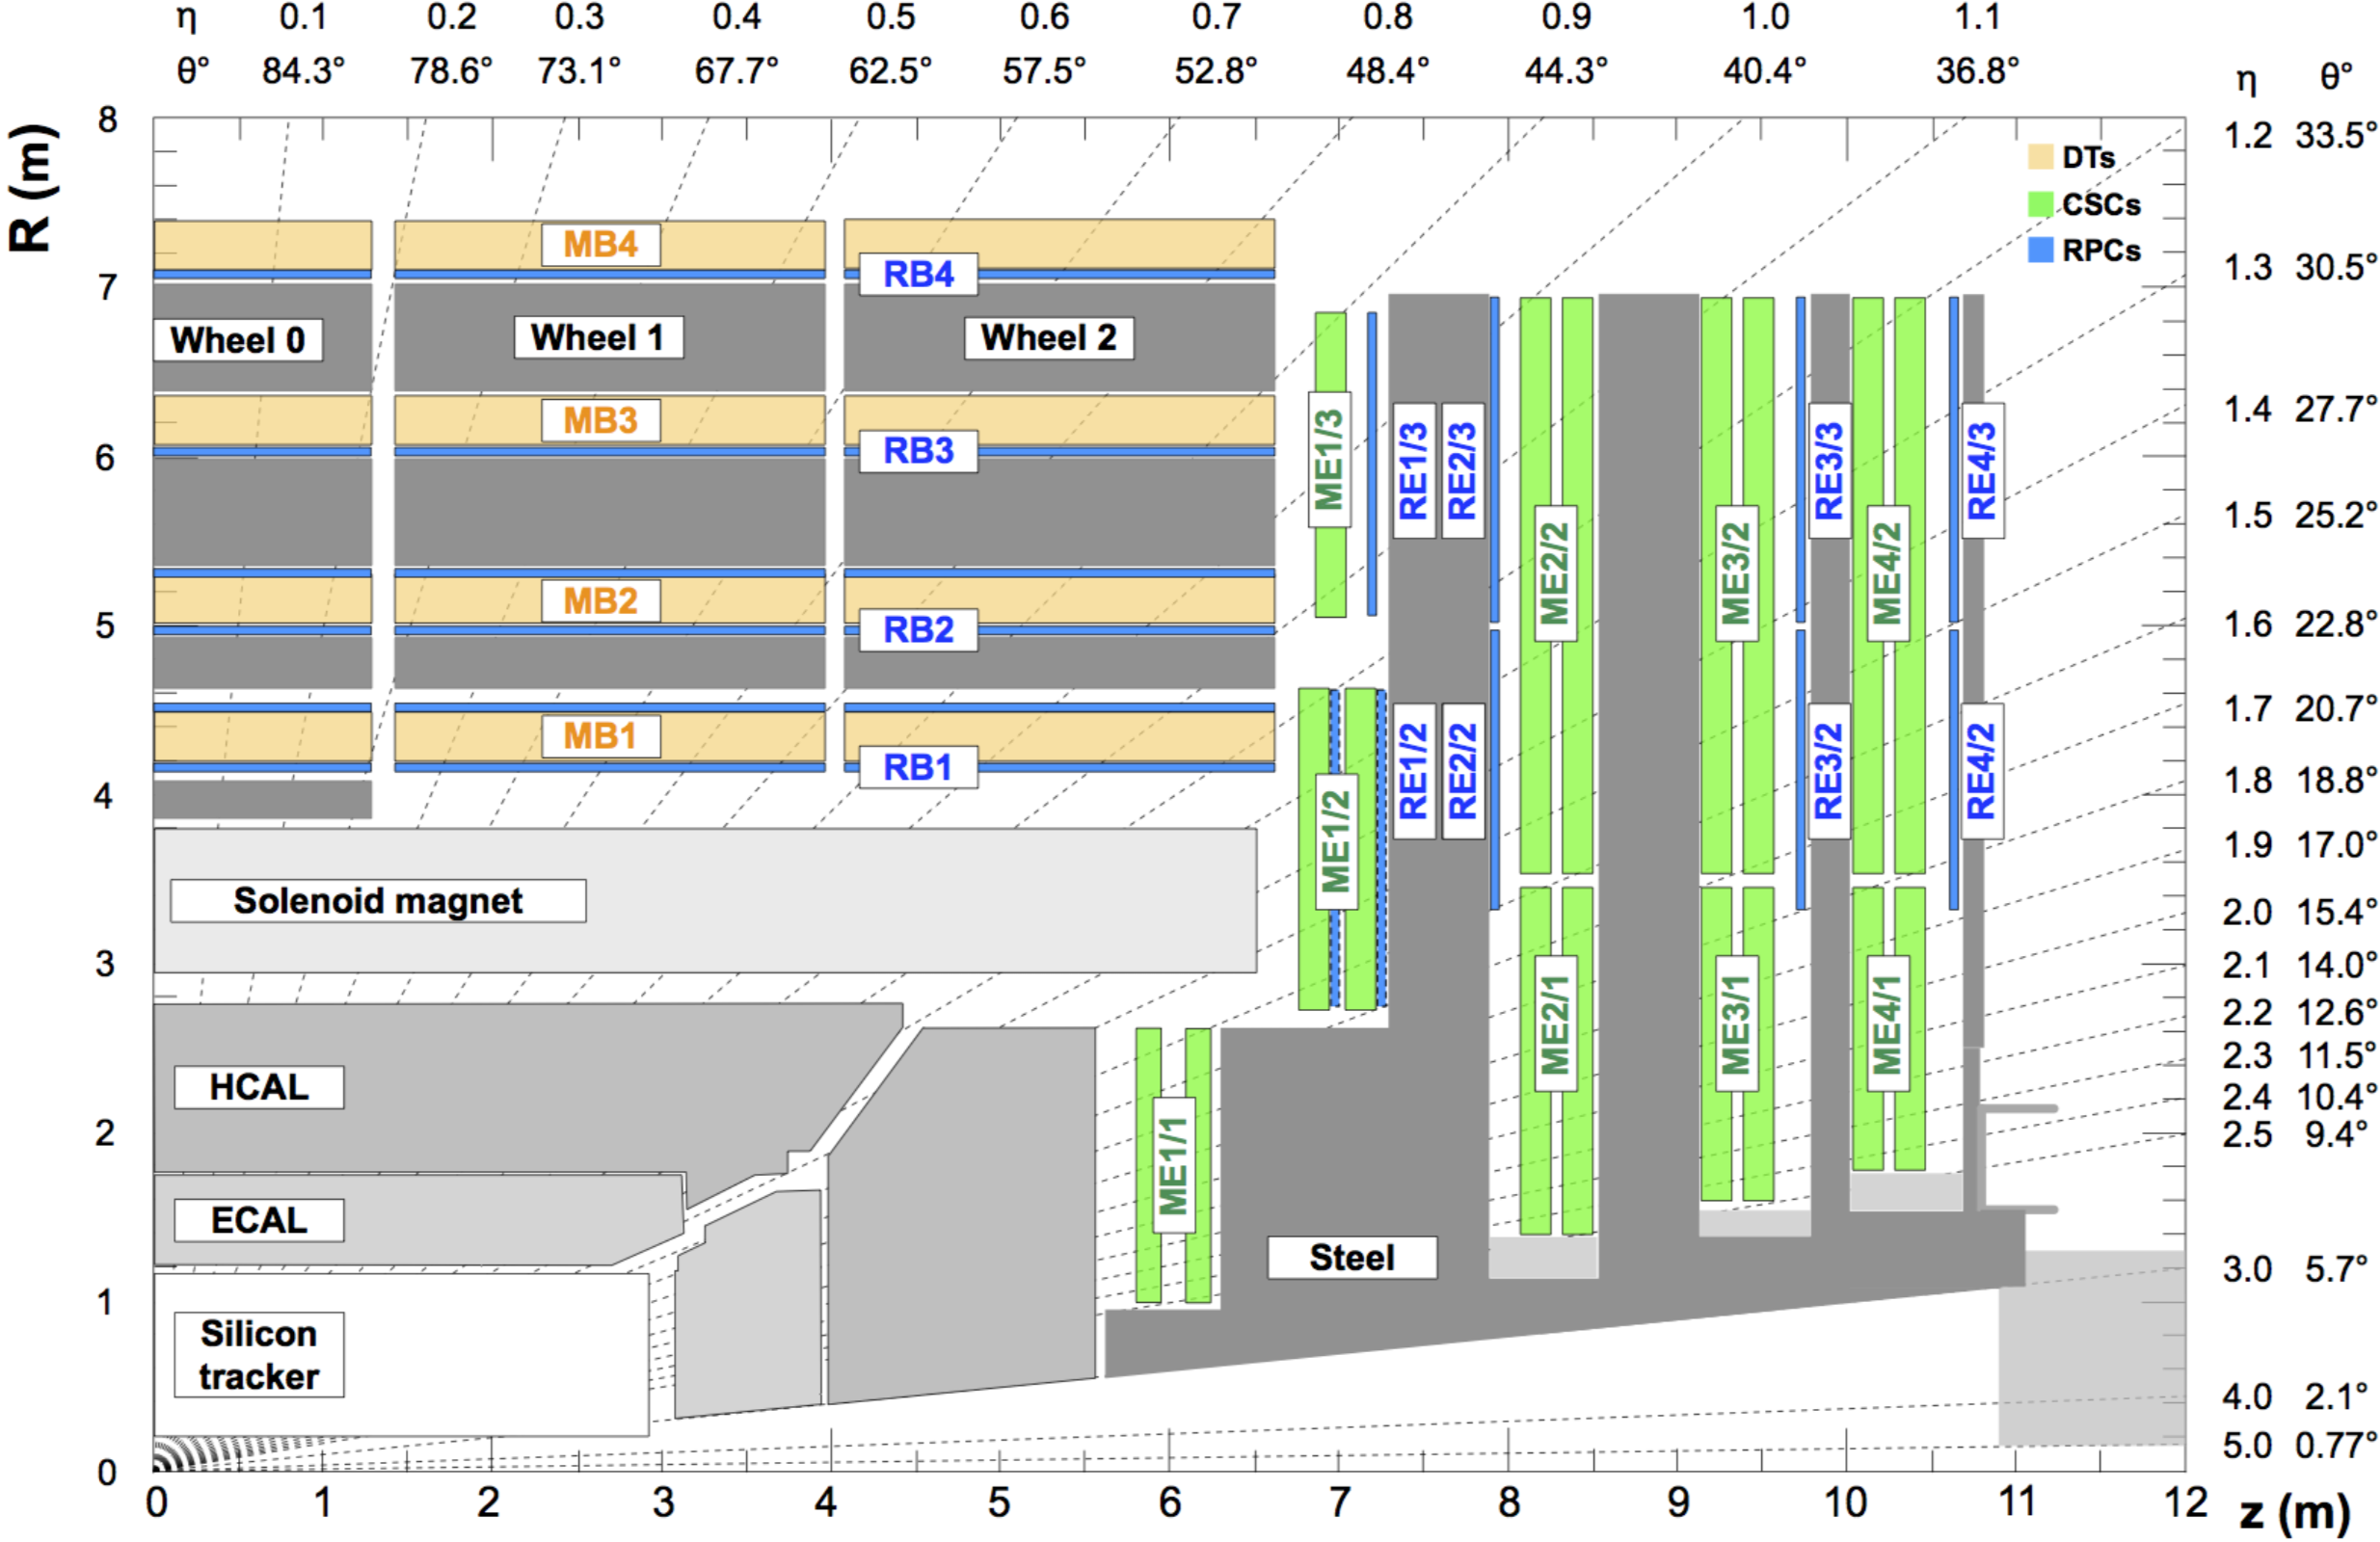
\includegraphics[width=5.5in]{images/muon_diagram}
    \caption[Schematic for the CMS Muon Subsystems]{A schematic diagram showing a cross sectional view of the CMS detector's muon subsystems in the positive $yz$-plane.\cite{MUONDIAGRAM}}
    \label{fig:CMSmuondiag}
\end{figure}

The muon subsystems form the outermost layer of the CMS detector and are designed to detect muons and measure their tracks. It is located far from the interaction point because the muon is a weakly interacting particle that easily penetrates through all preceding layers. While its function is similar to that of the silicon tracker, the muon subsystems eschew solid state for gas ionization chambers to accommodate the amount of surface area required to be covered. The muon subsystems are divided as shown in Figure \ref{fig:CMSmuondiag} into barrel ($\left| \eta \right| < 0.9$, overlap ($0.9 < \left| \eta \right| < 1.2$), and endcap ($1.2 < \left| \eta \right| < 2.5$) regions which deploy three different implementations of gas ionization chambers.

Drift tubes (DTs) are used in the barrel region because of the low muon rate and magnetic field. They are 4 cm wide tubes containing an anode wire and a gaseous mixture of argon and carbon dioxide with a ratio of 85\% to 15\%, respectively. The passage of a muon through the tube ionizes the gas molecules, whose electrons ``drift'' towards the anode wiring under the force of an applied electric field. The position of the muon is determined by the location of the signal along the wire and the travel time based on the drift velocity of electrons within the tube.

Cathode strip chambers (CSCs) are used in the endcap region because of the high muon rate and non-uniform magnetic field. These trapezoidal chambers are composed of six gaps filled with a gas mixture of 40\% argon, 50\% carbon dioxide, and 10\% carbon tetrafluoride ($CF_{4}$) that house planes of cathode strips oriented radially and anode wires oriented perpendicular to the strips. The passage of a muon through the chamber ionizes the gas molecules, with the electrons travelling to the anode wire and creating an avalanche of electrons and the positive ions travelling to the cathode strips and creating charge pulses. Because the wires and strips are perpendicular, the $r\phi$ position of the muon can be determined at six points and combined to form a track local to the chamber.

Resistive plate chambers (RPCs) are used both in the barrel and endcap regions, offering good spatial resolution and an xcellent time resolution of approximately 3 ns. They consist of two parallel plates made of a resin with high resistivity, one of which is an anode and the other a cathode. The plates surround a 2 mm wide gap filled with a gas mixture of 95\% tetrafluoroethane ($\mathrm{C_{2}H_{2}F_{4}}$) and 5\% isobutane ($\mathrm{i-C_{4}H_{10}}$). The passage of a muon through the chamber ionizes the gas molecules, producing an avalanche of electrons which are collected by metallic strips attached to one of the plates.

\subsection{Data Acquisition and Triggers}

At the LHC, approximately one billion proton-proton collisions occur each second and each hard scattering event takes on average one megabyte of storage, generating one petabyte of data every second. With contemporary particle detectors having data channels numbering in the millions, the volume of information is impossible to preserve. However, the vast majority of collision events are produced by common and well understood physics mechanisms rather than the rare processes which motivated the LHC's physics program. This observation informs the design of \textit{trigger} systems at the LHC experiments which are used to reduce the event rate by filtering for interesting signatures.

At the trigger level, low latencies are required to accomodate the 25 ns bunch crossing rate, which results in the overlap of particles from the current collision with those from the previous and next collisions. In order to maintain the trigger rates at acceptable levels, a hierarchical system of triggers is employed by the CMS experiment to filter events at the hardware and software levels. By implementing robust algorithms and taking advantage of data parallelism, the triggers are optimized and run extremely quickly. A full review of the data acquisition and trigger systems of the CMS experiment may be found in Ref. \cite{CMSTRIDAS}.

The \textit{Level 1 Trigger} (L1T) is the first stage of the trigger system used by the CMS experiment to filter events and is implemented in hardware processors with a fixed latency of 4 $\mu\mathrm{s}$. It consists of custom electronics, such as field-programmable gate arrays (FPGAs) and application-specific integrated circuits (ASICs), that are integrated with the calorimetry and muon subsystems. The decisions made by the L1T are based on the presence of \textit{trigger primitives} proposed by the detector subsystems, representing candidate particles such as muons or jets, which are processed individually and then evaluted as a whole by the global trigger (GT) for a final decision to accept or reject the event based on \pT\ and $E_{T}$ thresholds. If an event is accepted, the buffered information from the detector subsystems are read for offline storage. The L1T reduces the event rate from 40 MHz to a maximum of 100 kHz. An overview of the L1T is show in Figure \ref{fig:CMSL1T}.

\begin{figure}[htbp]
  \centering
    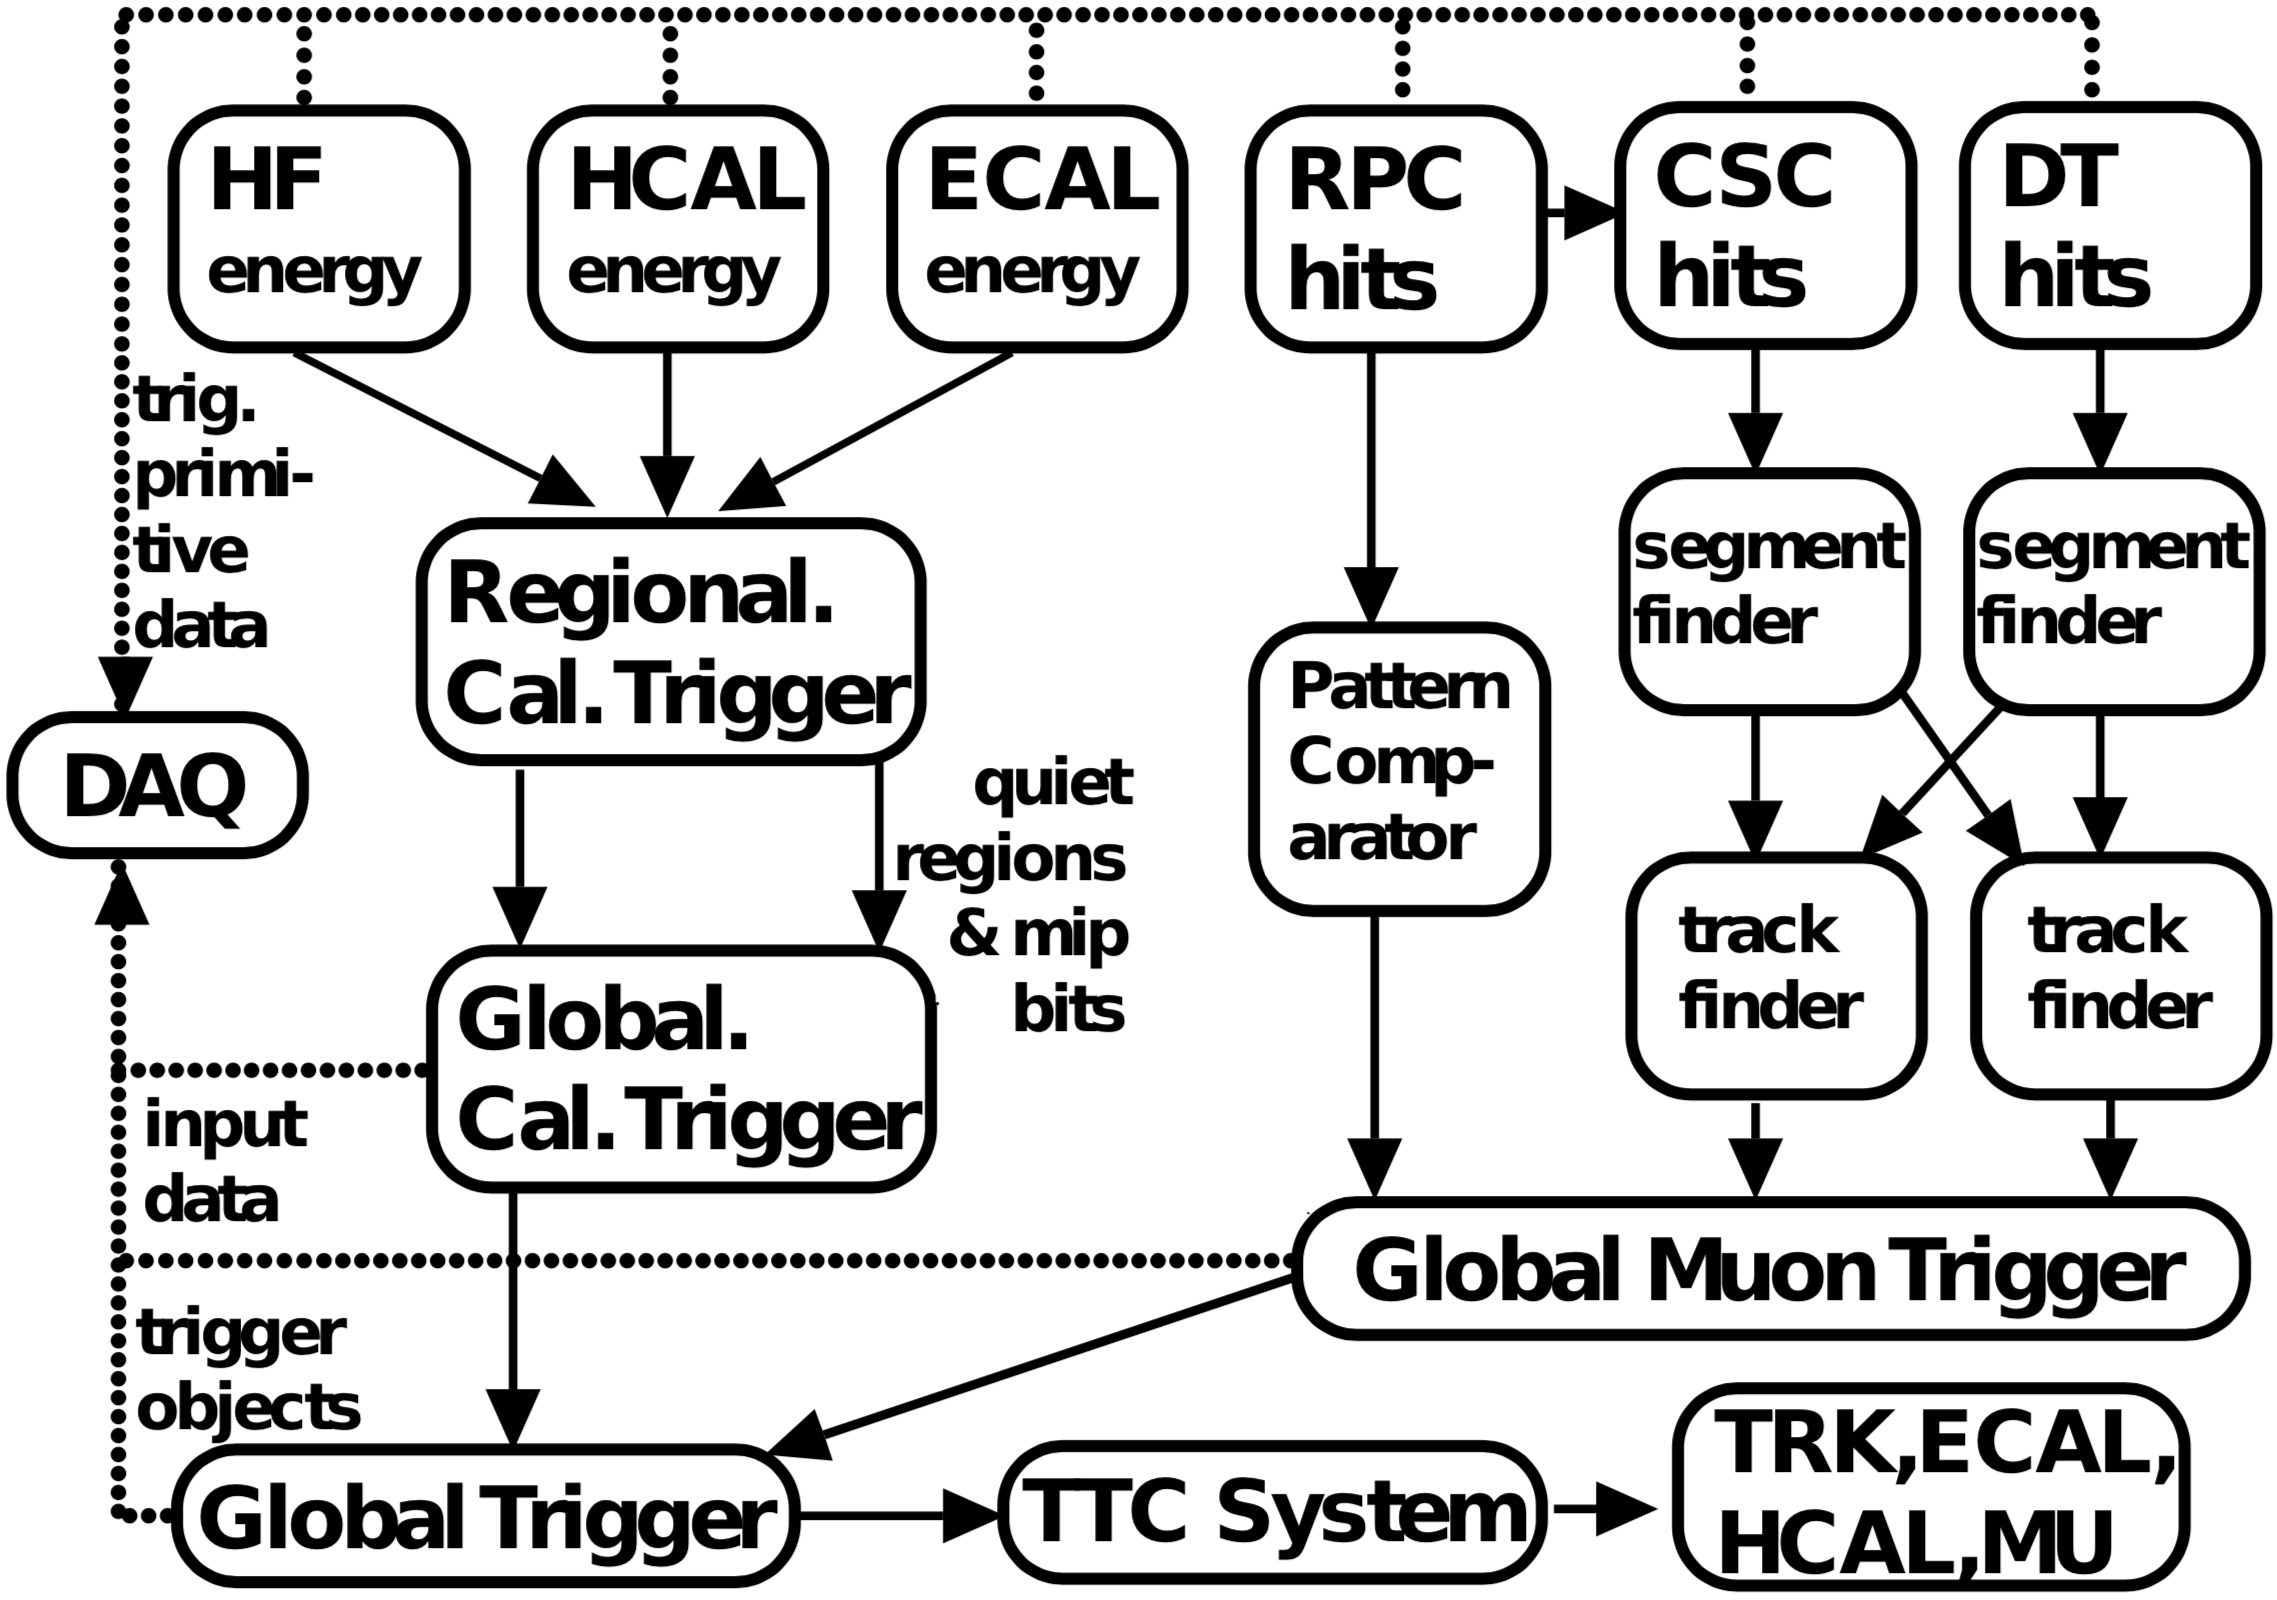
\includegraphics[width=3.5in]{images/l1t_overview}
    \caption[Overview of the Level 1 Trigger System]{An overview of the Level 1 Trigger System used by the CMS detector. The detector subsystems send trigger primitives to the DAQ and regional triggers. Global triggers for the calorimeter and muon subsystems then send data to the global trigger for the final decision to reject an event or accept it and release information buffered in the DAQ systems.\cite{CMSTRIDAS}}
    \label{fig:CMSL1T}
\end{figure}

The High Level Trigger (HLT), the second and last stage of the trigger system, is implemented in software that is executed on a computing cluster consisting of 26,000 cores. Because the algorithms use the full precision information recorded by the detector subsystems, the HLT has an average processing time of 260 ms per event.\cite{CMSHLT} There are several hundred algorithms, or \textit{HLT paths}, each designed for a particular physics goal and defining a sequence of modules that reconstruct objects of interest and performs selections based on their properties. If any modules reject the event, the remainder of the HLT path is short-circuited and the event is rejected. If an event is accepted, it is sent to the CMS Tier-0 computing center for storage and full event reconstruction. The HLT reduces the event rate from 100 kHz at the L1T level to around 100 Hz.

\subsection{Computing Resources}

In order to handle the computational requirements of the CMS experiment for tasks ranging from event reconstruction and storage to end-user data analysis, a distributed grid computing model is adopted. This computing infrastructure, known as the Worldwide LHC Computing Grid (WLCG), is a tiered system. The Tier-0 data center at CERN handles the reconstruction and long term storage of events. The data is transferred upon request to national laboratories and universities which host Tier-1 data centers located across Western Europe and in the United States and Taiwan and the smaller Tier-2 data centers used primarily for data analysis. A thorough review of the computing strategy is available in Ref. \cite{CMSCOMPUTE}.

%Many of the problems in theses and dissertations involve tables. The UF Graduate Counsel is very specific in the Table Requirements.\renewcommand*{\thefootnote}{\fnsymbol{footnote}}\footnote{an un-numbered footnote}\renewcommand*{\thefootnote}{\arabic{footnote}}\setcounter{footnote}{0}There should be no vertical lines in tables and only three horizontal lines. No bold text, etc., see the web site for the complete list of requirements.\footnote{and now we're back to normal footnote marking} One simple improvement can be incorporated by using tabularx instead of the tabular environment. This allows a table to be stretched the full text width easily, which avoids the centered or left aligned issue. \cite{garfinkle1991charged} Table \ref{first} is an examble of the tabularx code. Consectetur adipiscing elit. Fusce eget tempus lectus, non porttitor tellus. Aliquam molestie sed urna quis convallis. Aenean nibh eros, aliquam non eros in, tempus lacinia justo. In magna sapien, blandit a faucibus ac, scelerisque nec purus. 
% 
% \begin{table}[htbp]
%    \caption{A sample Table using tabularx}\label{first}
%    \begin{tabularx}{6.5in}{XXX}
%      \hline
%      First & Second & Third \\
%      \hline
%      12 & 45 & 26 \\
%      17 & 32 & 93 \\
%      text & 51 & can be there too. \\	
%      \epsfig{figure=images/cat.eps, scale=1} & 28 & Figures too - a cat. \\
%      \begin{turn}{0}\epsfig{figure=images/mouse.eps, scale=0.25}\end{turn} & 000 & and a mouse! \\
%      \hline
%    \end{tabularx}
%\end{table}
% 
% 
% Praesent fermentum felis nec massa interdum, vel dapibus mi luctus. Cras id fringilla mauris. Ut molestie eros mi, ut hendrerit nulla tempor et. Pellentesque tortor quam, mattis a scelerisque nec, euismod et odio. Mauris rhoncus metus sit amet risus mattis, eu mattis sem interdum.
%
% \begin{table}[htbp]
%    \caption{A sample Table using standard tablular}\label{first}
%    \begin{tabular}{c c c}
%      \hline
%      First & Second & Third \\
%      \hline
%      12 & 45 & 26 \\
%      17 & 32 & 93 \\
%      text & 51 & can be there too. \\	
%      \epsfig{figure=images/cat.eps, scale=1} & 28 & Figures too - a cat. \\
%      \begin{turn}{0}\epsfig{figure=images/mouse.eps, scale=0.25}\end{turn} & 000 & and a mouse! \\
%      \hline
%    \end{tabular}
%\end{table}
%
%\subsection{Platea Dictumst}
%Donec convallis scelerisque ante, in sollicitudin orci laoreet eu. Nam arcu magna, semper vel lorem eu, venenatis ultrices est. Nam aliquet ut erat ac scelerisque. Maecenas ut molestie mi. Phasellus ipsum magna, sollicitudin eu ipsum quis, imperdiet cursus turpis. Etiam pretium enim a fermentum accumsan. Morbi vel vehicula enim.
%
%
%\subsection{Long (and/or Wide) Tables}
%
%Another problem in LaTeX is the inability to handle long tables. While there are some packages that address this problem none of them quite fit the Editorial Office guidelines. The caption is not repeated but we do need "Table x-y. Continued" on each subsequent page and a repeat of the column headings on each page as well. The following table is the best example of the correct format I can produce. The disadvantage of this method is that much of it is manually set up and changes in the text will cause changes in the table. \citep{Moffatt69} For best results avoid the use of footnotemark and footnotetext commands inside of tables and try to keep your footnotes outside of floats whenever possible.
%
%
%
%\begin{table}
%\caption{Feasible triples for highly variable Grid, MLMMH.} \label{tbl1}
%\begin{tabularx}{6.5 in}{r l X}
%\hline {{Time (s)}} & {{Triple chosen}} & {{Other feasible triples}} \\ \hline
%0 & (1, 11, 13725) & (1, 12, 10980), (1, 13, 8235), (2, 2, 0), (3, 1, 0) \\
%2745 & (1, 12, 10980) & (1, 13, 8235), (2, 2, 0), (2, 3, 0), (3, 1, 0) \\
%5490 & (1, 12, 13725) & (2, 2, 2745), (2, 3, 0), (3, 1, 0) \\
%8235 & (1, 12, 16470) & (1, 13, 13725), (2, 2, 2745), (2, 3, 0), (3, 1, 0) \\
%10980 & (1, 12, 16470) & (1, 13, 13725), (2, 2, 2745), (2, 3, 0), (3, 1, 0) \\
%13725 & (1, 12, 16470) & (1, 13, 13725), (2, 2, 2745), (2, 3, 0), (3, 1, 0) \\
%16470 & (1, 13, 16470) & (2, 2, 2745), (2, 3, 0), (3, 1, 0) \\
%19215 & (1, 12, 16470) & (1, 13, 13725), (2, 2, 2745), (2, 3, 0), (3, 1, 0) \\
%21960 & (1, 12, 16470) & (1, 13, 13725), (2, 2, 2745), (2, 3, 0), (3, 1, 0) \\
%24705 & (1, 12, 16470) & (1, 13, 13725), (2, 2, 2745), (2, 3, 0), (3, 1, 0) \\
%27450 & (1, 12, 16470) & (1, 13, 13725), (2, 2, 2745), (2, 3, 0), (3, 1, 0) \\
%30195 & (2, 2, 2745) & (2, 3, 0), (3, 1, 0) \\
%32940 & (1, 13, 16470) & (2, 2, 2745), (2, 3, 0), (3, 1, 0) \\
%35685 & (1, 13, 13725) & (2, 2, 2745), (2, 3, 0), (3, 1, 0) \\
%38430 & (1, 13, 10980) & (2, 2, 2745), (2, 3, 0), (3, 1, 0) \\
%41175 & (1, 12, 13725) & (1, 13, 10980), (2, 2, 2745), (2, 3, 0), (3, 1, 0) \\
%43920 & (1, 13, 10980) & (2, 2, 2745), (2, 3, 0), (3, 1, 0) \\
%46665 & (2, 2, 2745) & (2, 3, 0), (3, 1, 0) \\
%49410 & (2, 2, 2745) & (2, 3, 0), (3, 1, 0) \\
%52155 & (1, 12, 16470) & (1, 13, 13725), (2, 2, 2745), (2, 3, 0), (3, 1, 0) \\
%54900 & (1, 13, 13725) & (2, 2, 2745), (2, 3, 0), (3, 1, 0) \\
%57645 & (1, 13, 13725) & (2, 2, 2745), (2, 3, 0), (3, 1, 0) \\
%60390 & (1, 12, 13725) & (2, 2, 2745), (2, 3, 0), (3, 1, 0) \\
%63135 & (1, 13, 16470) & (2, 2, 2745), (2, 3, 0), (3, 1, 0) \\
%65880 & (1, 13, 16470) & (2, 2, 2745), (2, 3, 0), (3, 1, 0) \\
%68625 & (2, 2, 2745) & (2, 3, 0), (3, 1, 0) \\
%71370 & (1, 13, 13725) & (2, 2, 2745), (2, 3, 0), (3, 1, 0) \\
%74115 & (1, 12, 13725) & (2, 2, 2745), (2, 3, 0), (3, 1, 0) \\
%76860 & (1, 13, 13725) & (2, 2, 2745), (2, 3, 0), (3, 1, 0) \\
%79605 & (1, 13, 13725) & (2, 2, 2745), (2, 3, 0), (3, 1, 0) \\
%82350 & (1, 12, 13725) & (2, 2, 2745), (2, 3, 0), (3, 1, 0) \\
%85095 & (1, 12, 13725) & (1, 13, 10980), (2, 2, 2745), (2, 3, 0), (3, 1, 0) \\
%87840 & (1, 13, 16470) & (2, 2, 2745), (2, 3, 0), (3, 1, 0) \\
%90585 & (1, 13, 16470) & (2, 2, 2745), (2, 3, 0), (3, 1, 0) \\
%93330 & (1, 13, 13725) & (2, 2, 2745), (2, 3, 0), (3, 1, 0) \\
%96075 & (1, 13, 16470) & (2, 2, 2745), (2, 3, 0), (3, 1, 0) \\
%98820 & (1, 13, 16470) & (2, 2, 2745), (2, 3, 0), (3, 1, 0) \\
%101565 & (1, 13, 13725) & (2, 2, 2745), (2, 3, 0), (3, 1, 0) \\
%104310 & (1, 13, 16470) & (2, 2, 2745), (2, 3, 0), (3, 1, 0) \\
%107055 & (1, 13, 13725) & (2, 2, 2745), (2, 3, 0), (3, 1, 0) \\
%109800 & (1, 13, 13725) & (2, 2, 2745), (2, 3, 0), (3, 1, 0) \\
%112545 & (1, 12, 16470) & (1, 13, 13725), (2, 2, 2745), (2, 3, 0), (3, 1, 0) \\
%\hline
%\end{tabularx}
%\end{table}
%
%\begin{table}[h!t!]
%\begin{tabularx}{6.5 in}{r l X}
%\multicolumn{3}{l}{Table \ref{tbl1}. Continued}\\%
%\hline {{Time (s)}} & {{Triple chosen}} & {{Other feasible triples}} \\ \hline
%115290 & (1, 13, 16470) & (2, 2, 2745), (2, 3, 0), (3, 1, 0) \\
%118035 & (1, 13, 13725) & (2, 2, 2745), (2, 3, 0), (3, 1, 0) \\
%120780 & (1, 13, 16470) & (2, 2, 2745), (2, 3, 0), (3, 1, 0) \\
%123525 & (1, 13, 13725) & (2, 2, 2745), (2, 3, 0), (3, 1, 0) \\
%126270 & (1, 12, 16470) & (1, 13, 13725), (2, 2, 2745), (2, 3, 0), (3, 1, 0) \\
%129015 & (2, 2, 2745) & (2, 3, 0), (3, 1, 0) \\
%131760 & (2, 2, 2745) & (2, 3, 0), (3, 1, 0) \\
%134505 & (1, 13, 16470) & (2, 2, 2745), (2, 3, 0), (3, 1, 0) \\
%137250 & (1, 13, 13725) & (2, 2, 2745), (2, 3, 0), (3, 1, 0) \\
%139995 & (2, 2, 2745) & (2, 3, 0), (3, 1, 0) \\
%142740 & (2, 2, 2745) & (2, 3, 0), (3, 1, 0) \\
%145485 & (1, 12, 16470) & (1, 13, 13725), (2, 2, 2745), (2, 3, 0), (3, 1, 0)\\%
%148230 & (2, 2, 2745) & (2, 3, 0), (3, 1, 0) \\
%150975 & (1, 13, 16470) & (2, 2, 2745), (2, 3, 0), (3, 1, 0) \\
%153720 & (1, 12, 13725) & (2, 2, 2745), (2, 3, 0), (3, 1, 0) \\
%156465 & (1, 13, 13725) & (2, 2, 2745), (2, 3, 0), (3, 1, 0) \\
%159210 & (1, 13, 13725) & (2, 2, 2745), (2, 3, 0), (3, 1, 0) \\
%161955 & (1, 13, 16470) & (2, 2, 2745), (2, 3, 0), (3, 1, 0) \\
%164700 & (1, 13, 13725) & (2, 2, 2745), (2, 3, 0), (3, 1, 0) \\
%\hline
%\end{tabularx}
%\end{table}
%
%\section{Ex id ullamcorper commodo}
%Augue sapien mattis leo, nec accumsan turpis quam at neque. Ut pellentesque velit sed placerat cursus. Integer congue urna non massa dictum, a pellentesque arcu accumsan. Nulla posuere, elit accumsan eleifend elementum, ipsum massa tristique metus, in ornare neque nisl sed odio. Nullam eget elementum nisi. Duis a consectetur erat, sit amet malesuada sapien. Aliquam nec sapien et leo sagittis porttitor at ut lacus. Vivamus vulputate elit vitae libero condimentum dictum. Nulla facilisi. Quisque non nibh et massa ullamcorper iaculis.
%
%Integer laoreet bibendum arcu non pulvinar. Curabitur ac magna nibh. Phasellus sed nisi semper, molestie neque at, tempus lacus. Aenean vitae lacinia est. Phasellus aliquam lacus sit amet placerat molestie. Sed sit amet bibendum lectus, ac ornare ligula. Curabitur porttitor interdum tortor a dignissim. Quisque a placerat nibh. Phasellus lobortis imperdiet augue, non congue est bibendum eu. Vivamus tincidunt quam eu fringilla laoreet.
%
%Maecenas efficitur dolor et ipsum convallis, ut fringilla neque luctus. Donec ac nisl quis leo gravida accumsan sit amet sed tellus. Quisque placerat hendrerit augue sit amet aliquet. Vestibulum laoreet consequat nunc, et egestas nisl auctor et. Duis scelerisque vulputate placerat. Proin tempus ligula ac tempor eleifend. Nullam est odio, commodo quis nisl eu, feugiat efficitur purus.
%
%Duis egestas in mauris vel efficitur. Sed a faucibus sem, non euismod enim. Maecenas nec nulla justo. Suspendisse ut orci ac mi aliquet tincidunt ac eget quam. Quisque ac mi sagittis, dapibus dui a, facilisis neque. Aenean euismod orci sem, non imperdiet ipsum pulvinar ac. Proin eu vestibulum magna, eu ullamcorper nulla. Etiam enim felis, dignissim eget commodo ac, faucibus nec justo. Nulla condimentum velit imperdiet ligula aliquam semper. Nulla facilisi. Ut in lobortis metus, at dictum ipsum. Suspendisse facilisis nec eros eget mollis. Vestibulum eget dolor ac mauris lobortis gravida. Suspendisse consectetur orci in risus pharetra, sed eleifend nisl lacinia. Mauris augue nibh, commodo sed sem at, congue molestie massa. Suspendisse sodales aliquet tellus, a tristique nunc aliquam id.

